\documentclass[11pt]{article}
\usepackage[margin=0.85in]{geometry}
\usepackage{amsmath,amssymb,booktabs,graphicx,hyperref,xurl,longtable,array}
\hypersetup{colorlinks=true,linkcolor=blue,citecolor=blue,urlcolor=blue}
\setlength{\parskip}{0.45em}
\setlength{\parindent}{0pt}
\title{Full Derivation Ledger for the Branch A Higgs Module}
\author{Jozsef Olcsak}
\date{May 20, 2026}
\begin{document}
\maketitle

\begin{abstract}
This companion ledger expands the derivation chain behind Paper 4.  It is not
an empirical paper, not a complete Standard Model derivation, and not a claim
that the Higgs sector has been solved.  Its purpose is to collect the working
Branch A gate stack in one generated PDF: stabilizer normalization,
localization forcing, quartic overlap, Yukawa product, bridge-trace
normalization, v0.2 single-package parent action, absolute-scale gate,
wall-cell embedding, and the remaining top/BRST/regulator blockers.
\end{abstract}

\tableofcontents

\section{Status Discipline}
This ledger uses four statuses.

\begin{longtable}{p{0.22\linewidth}p{0.68\linewidth}}
\toprule
\textbf{Status} & \textbf{Meaning}\\
\midrule
Derived in gate & Follows inside the stated Branch A assumptions or audit.\\
Theorem-candidate & Would become a theorem if the listed parent conditions are derived.\\
Open gate & Required before a physical claim can be made.\\
Forbidden overclaim & A claim explicitly not licensed by the current construction.\\
\bottomrule
\end{longtable}

The guiding rule is simple: no quantity may be chosen from the observed Higgs
vev, measured Higgs mass, or top mass and then presented as derived.

\section{Global Dependency Chain}
The current Higgs-route dependency chain is
\begin{equation}
3+2
\rightarrow
T_Y
\rightarrow
\kappa_\tau^2=\frac35
\rightarrow
Q_i=\partial_x+\kappa_\tau^2Y_i\tanh x
\rightarrow
\nu_i=\kappa_\tau^2|Y_i|
\rightarrow
I_4(3/10)
\rightarrow
{\cal I}_{qHu}
\rightarrow
y_t^{\rm parent}
\rightarrow
\Lambda_A
\rightarrow
m_t^{\rm candidate}.
\end{equation}
The first part is dimensionless and comparatively sharp.  The last part is a
scale/matching problem and remains open.

\section{Branch A Stabilizer And Hypercharge Normalization}
Start from the visible carrier
\begin{equation}
V\simeq \mathbb{C}^5=C\oplus W,
\qquad
\dim C=3,
\quad
\dim W=2.
\end{equation}
The traceless two-block generator is
\begin{equation}
T_\Sigma=\frac1{\sqrt{60}}{\rm diag}(2,2,2,-3,-3).
\end{equation}
The stabilizer is $S(U(3)\times U(2))$.  A stabilizer-preserving Abelian
connection must be block-scalar:
\begin{equation}
T={\rm diag}(a,a,a,b,b),
\qquad
3a+2b=0.
\end{equation}
Thus the traceless centralizer is one-dimensional.  Choosing the conventional
hypercharge orientation gives
\begin{equation}
Y={\rm diag}\left(-\frac13,-\frac13,-\frac13,\frac12,\frac12\right),
\qquad
T_Y=\sqrt{\frac35}Y,
\end{equation}
and $T_\Sigma=-T_Y$.  The Branch A normalization is therefore
\begin{equation}
\kappa_\tau^2=\frac35.
\end{equation}
This is not fitted to the Higgs quartic.  It comes from canonical normalization
of the unique traceless Abelian line in the $3+2$ stabilizer.

\section{Spectral Origin Of The Normalization Gate}
The next upgrade is to derive the same coefficient from the compact spectral
geometry rather than from a normalization convention.  In the v0.1 compact
geometry, the target is
\begin{equation}
\kappa_\tau^2
=
\frac{\operatorname{Tr}_{\cal F}(T_Y^2)}{\operatorname{Tr}_{\cal F}(Y^2)}
=\frac35 ,
\end{equation}
where the finite fiber ${\cal F}=\mathbb C^3\oplus\mathbb C^2$ and trace
functional are selected by the compact domain.  A more intrinsic version would
express the same value as a heat-kernel or index residue:
\begin{equation}
\kappa_\tau^2
\sim
\frac{\operatorname{Res}_{s=0}\operatorname{Tr}(T_Y^2|D_\tau|^{-s})}
{\operatorname{Res}_{s=0}\operatorname{Tr}(Y^2|D_\tau|^{-s})} .
\end{equation}
The proof obligation is therefore:
\begin{enumerate}
\item the compact spectrum must select the trace functional;
\item the protected hypercharge line must be an eigenline or index residue of
the compact operator;
\item the residue ratio must be stable under allowed regulator choices;
\item no alternative Abelian line may give a lower selection penalty.
\end{enumerate}
If this closes, the factor $3/5$ becomes a spectral number of the compact
geometry.  Combined with the charge-to-exponent theorem target, this would turn
$\nu_D=3/10$ into a genuine geometric/spectral consequence rather than a
conditional Branch A input.

\section{Unoriented Line And Two-Vacuum Quotient}
The Branch A Abelian direction is treated as an internal line rather than as a
signed observable vector:
\begin{equation}
L_Y={\rm span}(T_Y).
\end{equation}
If the regular parent datum is the line or projector, then
\begin{equation}
{\rm span}(T_Y)={\rm span}(-T_Y),
\qquad
P_Y=P_{-Y},
\qquad
\Sigma\sim-\Sigma.
\end{equation}
For $\Sigma=fT_Y$, sign-even invariants satisfy
\begin{equation}
{\rm Tr}(\Sigma^2)=\frac12 f^2,
\qquad
{\rm Tr}(\Sigma'^2)=\frac12(f')^2.
\end{equation}
If the regular branch fixes $2{\rm Tr}(\Sigma^2)=1$, then $f^2=1$ and the
two oriented representatives are $f=\pm1$.  This gives the two-vacuum logic
conditional on the parent deriving the unoriented-line/projector quotient.

\section{Minimal Wall Profile}
The leading local two-vacuum wall is modeled by the BPS equation
\begin{equation}
f'(x)=1-f(x)^2,
\end{equation}
whose centered solution is
\begin{equation}
f(x)=\tanh x.
\end{equation}
Equivalently, it is generated by
\begin{equation}
V(f)=\frac12(1-f^2)^2.
\end{equation}
The wall is not selected to fit the Higgs quartic.  The open parent-level task
is to derive this minimal BPS functional and forbid leading deformations that
change the localization rule.

\section{Localization Derivation}
Given the selected hypercharge wall line, the local first-order operator is
\begin{equation}
Q_i=\partial_x+\kappa_\tau^2Y_i\tanh x.
\end{equation}
The zero-mode equation gives
\begin{align}
Q_i h_i&=0,\\
\partial_x h_i&=-\kappa_\tau^2Y_i\tanh x\,h_i,\\
h_i(x)&\propto
\exp\left[-\int^x\kappa_\tau^2Y_i\tanh u\,du\right]
={\rm sech}^{\kappa_\tau^2Y_i}x.
\end{align}
Normalizability selects the chirality/sign, so
\begin{equation}
\nu_i=\kappa_\tau^2|Y_i|.
\end{equation}
For the Higgs doublet,
\begin{equation}
\nu_H=\frac35\left|\frac12\right|=\frac3{10}.
\end{equation}
This is the current natural-origin derivation.  It becomes a proof only when
the parent action derives the wall line, BPS wall, same-domain Hessian, and
chiral admissibility.

\section{Charge-To-Exponent Theorem Target}
The value $\nu_H=3/10$ has two ingredients.  The first is already algebraic:
canonical Branch A normalization gives
\begin{equation}
\kappa_\tau^2=\frac35,\qquad |Y_D|=\frac12 .
\end{equation}
The second is still the hard gate: the compact geometry must show that the
wall connection seen by a component with hypercharge $Y_i$ is exactly
\begin{equation}
A_{\tau,i}(x)=\kappa_\tau^2Y_i f(x)
\end{equation}
on the self-adjoint wall domain.  If this is derived, the first-order local
operator is forced:
\begin{equation}
Q_i=\partial_x+A_{\tau,i}(x),
\qquad
Q_i h_i=0 .
\end{equation}
For the Bogomolny wall $f(x)=\tanh x$,
\begin{equation}
h_i(x)\propto
\exp\left[-\kappa_\tau^2Y_i\int^x\tanh u\,du\right]
=\operatorname{sech}^{\kappa_\tau^2Y_i}x,
\end{equation}
and normalizability gives
\begin{equation}
\nu_i=\kappa_\tau^2|Y_i|.
\end{equation}

Therefore the derivation problem is now sharply localized.  One must prove
that the compact spectral geometry selects a universal hypercharge-line
connection coefficient $\kappa_\tau^2=3/5$ and forbids extra component-dependent
connection terms:
\begin{equation}
A_{\tau,i}(x)\neq
\kappa_\tau^2Y_i f(x)+\delta A_i(x)
\end{equation}
unless $\delta A_i$ is Q-exact, quotient-null, or massive/leakage-suppressed.
This is the precise theorem that would turn the current $3/10$ input into a
geometric/spectral consequence.

\section{F1--F8 Forcing Theorem Candidate}
The stronger theorem-candidate says the localization rule is forced if the
parent action derives F1--F8.

\begin{longtable}{p{0.10\linewidth}p{0.36\linewidth}p{0.42\linewidth}}
\toprule
\textbf{Gate} & \textbf{Requirement} & \textbf{Consequence}\\
\midrule
F1 & quotient-visible trace removal & identity direction cannot become a wall channel\\
F2 & two protected visible blocks & exactly two low-energy visible modules\\
F3 & stabilizer-preserving wall & wall is block-scalar\\
F4 & one traceless Abelian wall line & no extra Abelian wall freedom\\
F5 & universal trace pairing & fixes $\kappa_\tau^2=3/5$\\
F6 & unoriented two-vacuum quotient & gives the $\pm$ wall representatives\\
F7 & minimal BPS factorization & gives leading $f=\tanh x$\\
F8 & same-domain Hessian/Q factorization & forbids importing $Q_i$ by hand\\
\bottomrule
\end{longtable}

Under these conditions the operator $Q_i$ and the exponent $\nu_i$ follow at
leading order.  Still open: deriving F1--F8 from the final parent action and
stationary background.

\section{Minimal Forcing Parent-Action Candidate}
The current action-level scaffold behind F1--F8 contains:
\begin{itemize}
\item trace projection $\Pi_{\rm tr}$ to remove the identity direction;
\item a stabilizer-stratified wall sector;
\item positive transverse/off-block gaps;
\item an unoriented-line quotient sector;
\item a minimal BPS wall term;
\item a same-domain Hessian/Q admissibility term.
\end{itemize}
It forces the trace quotient, trace pairing, leading BPS wall, and local
localization consequence at gate level.  It does not yet fully force the two
protected visible modules, the deep origin of the unoriented-line quotient, or
continuum QFT closure.

\section{Quartic Overlap Calculation}
For
\begin{equation}
h_\nu(x)=N_\nu{\rm sech}^{\nu}x,
\qquad
\int h_\nu^2dx=1,
\end{equation}
the normalization is
\begin{equation}
N_\nu^2=\frac{\Gamma(\nu+1/2)}{\sqrt\pi\Gamma(\nu)}.
\end{equation}
The quartic overlap is
\begin{equation}
I_4(\nu)
=
\frac{\Gamma(\nu+1/2)^2\Gamma(2\nu)}
{\sqrt\pi\Gamma(\nu)^2\Gamma(2\nu+1/2)}.
\end{equation}
At $\nu_H=3/10$,
\begin{equation}
I_4(3/10)=0.133756368895144.
\end{equation}
For $\lambda_H\simeq0.129$,
\begin{equation}
\lambda_\tau\simeq 0.964440057.
\end{equation}
The safe claim is order-one parent quartic, not a derived canonical quartic.

\section{Sensitivity Audit}
The generator also writes a sensitivity audit.  In the moderate window
$0.25\leq\nu\leq0.35$, the required parent quartic remains order one.  This
reduces numerology risk: the mechanism is not a delta-function coincidence at
$\nu=0.3$.  The audit still does not prove the localization rule.

\section{Yukawa Product Cohomology Gate}
The up-type slot is treated as a parent cohomology product, not a post-hoc
operator insertion:
\begin{equation}
[q_L]\,[H]\,[u_R^c].
\end{equation}
It is admissible only if it is neutral, bridge-closed, Q-closed modulo Q-exact
terms, and defined on the same Branch A domain as the wall/Hessian package.
The gate does not derive family hierarchy or the measured top mass.

\section{Yukawa Overlap}
The fixed exponents are
\begin{equation}
\nu_q=\frac1{10},
\qquad
\nu_H=\frac3{10},
\qquad
\nu_u=\frac25.
\end{equation}
With
\begin{equation}
I(a)=\int_{\mathbb R}{\rm sech}^a x\,dx
=\sqrt\pi\frac{\Gamma(a/2)}{\Gamma((1+a)/2)},
\end{equation}
the normalized overlap is
\begin{equation}
{\cal I}_{qHu}
=
N_{\nu_q}N_{\nu_H}N_{\nu_u}
I(\nu_q+\nu_H+\nu_u)
=
0.267097842200176.
\end{equation}
This is reproducible and endpoint-free.

\section{$g_t$ Bridge-Trace Normalization}
The current normalization theorem-candidate sums over the full $3\times2$
shared bridge and multiplies by the canonical wall coupling:
\begin{equation}
g_t=(3\times2)\kappa_\tau^2=6\cdot\frac35=\frac{18}{5}.
\end{equation}
Therefore
\begin{equation}
y_t^{\rm parent}
=g_t{\cal I}_{qHu}
=0.961552231920634.
\end{equation}
This is close to an order-one top Yukawa, but it is not a top-mass prediction.
The measured value still requires $v_{\rm eff}$, $R_t$, family selection,
and QFT matching.

\section{$v_{\rm eff}$ From Stabilizer Gap}
The current electroweak-scale gate proposes
\begin{equation}
v_{\rm eff}=\frac{M_{\rm stab}}{g_{\rm vis}}.
\end{equation}
Here $M_{\rm stab}$ must be the parent-derived positive Hessian/stabilizer
gap protecting the Higgs-like residue, and $g_{\rm vis}$ must be a universal
visible gauge normalization.  This is better than inserting $246$ GeV, but it
is not yet a derivation of the measured vev.

\section{Running And Matching}
The admissible matching factor is
\begin{equation}
R_t=R_{\rm match}R_{\rm run},
\qquad
R_{\rm run}=\exp\left[-\int \gamma_t(\mu)d\ln\mu\right].
\end{equation}
This is a shape requirement only.  $\gamma_t$, $R_{\rm match}$, regulator,
and matching scale must come from the same QFT closure before a physical top
mass can be claimed.

\section{Physical Matching Admissibility Map}
The physical matching problem is now a forward map, not a backsolve:
\begin{equation}
S_{\rm parent}
\longrightarrow
(\epsilon_\tau,C_A,\mu_\tau({\cal K}_\tau),N_\tau,\hat E_{\rm wall})
\longrightarrow
\Lambda_A
\longrightarrow
(v_{\rm eff},y_t^{\rm phys},m_H,m_t,\Delta g/g).
\end{equation}
The forbidden reverse map is
\begin{equation}
(v_{\rm obs},m_H^{\rm obs},m_t^{\rm obs})
\not\Longrightarrow
(\epsilon_\tau,C_A,R_t).
\end{equation}
Thus physical matching is admissible only if the absolute scale, running,
threshold correction, and visible gauge normalization are fixed upstream of
the measured Higgs and top endpoints.  A successful matching calculation may
compare to the measured vev, Higgs mass, top mass, and collider coupling
constraints, but it may not use those numbers to define the parent scale or
the top matching factor.

\section{Numerical Endpoint Matching Protocol}
The endpoint comparison can also be made falsifiable before it is executed.
Once the parent calculation outputs
\begin{equation}
\Theta_{\rm pred}
=
(\epsilon_\tau,C_A,\mu_\tau,N_\tau,\hat E_{\rm wall},
R_t^{\rm fin},Z_H,Z_t),
\end{equation}
the matching code must freeze these numbers and compute
\begin{equation}
{\cal M}(\Theta_{\rm pred})
=
(v_{\rm eff},m_H,m_t,\Delta g_H,\Delta g_t).
\end{equation}
Only then may the result be compared with the observed endpoint vector
\begin{equation}
{\cal E}_{\rm obs}
=
(v_{\rm obs},m_H^{\rm obs},m_t^{\rm obs},
\Delta g_H^{\rm obs},\Delta g_t^{\rm obs}).
\end{equation}
The pass/fail statistic should be declared before looking at the residuals,
for example
\begin{equation}
\chi_{\rm end}^2
=
({\cal M}(\Theta_{\rm pred})-{\cal E}_{\rm obs})^T
\Sigma_{\rm obs}^{-1}
({\cal M}(\Theta_{\rm pred})-{\cal E}_{\rm obs}).
\end{equation}
This does not perform numerical endpoint matching.  It defines the allowed
order of operations: derive, freeze, run, compare.  Any workflow that adjusts
$\epsilon_\tau$, $C_A$, $R_t^{\rm fin}$, or $Z_H$ after seeing the endpoint
residuals is a failed matching protocol, even if the final numbers look good.

\section{Dimensional Obstruction}
The Branch A action currently fixes dimensionless data.  A dimensionless action
cannot output an absolute GeV scale.  Therefore
\begin{equation}
\Lambda_A=s_A\hat E_{\rm wall}
\end{equation}
requires one remaining absolute unit $s_A$.

\section{$s_A$ And Compact Tau-Cell Unit}
The most native route is
\begin{equation}
s_A=C_AE_\tau,
\qquad
E_\tau=\epsilon_\tau\mu_\tau({\cal K}_\tau)N_\tau.
\end{equation}
This route is admissible only if the compact cell, its measure, the count/index
density, and $\epsilon_\tau$ are selected before Higgs/top comparison.

\section{Compact Tau Geometry Target}
The compact cell must become a concrete object rather than a name.  The
minimal target data are
\begin{equation}
({\cal K}_\tau,{\cal A}_\tau,{\cal H}_\tau,D_\tau,\mu_\tau),
\end{equation}
where ${\cal A}_\tau$ is an internal algebra, ${\cal H}_\tau$ is the
domain, $D_\tau$ is the spectral operator, and $\mu_\tau$ is the trace or
measure.  A useful candidate must produce the Branch A wall as a defect,
quotient, or induced Hessian sector of this same package:
\begin{equation}
{\cal W}_A={\rm Defect}({\cal K}_\tau,D_\tau,T_Y)
\quad{\rm or}\quad
{\cal W}_A={\cal K}_\tau/{\cal H}_A .
\end{equation}
The decisive check is whether the low-lying spectral/Hessian data of
${\cal K}_\tau$ select $3+2$, the hypercharge line, a two-vacuum kink, the
same-domain $Q$ package, and a finite determinant regulator without inserting
those choices by hand.

\section{C0 Finite-Fiber Wall Spectral Cell}
The first explicit compact-geometry candidate uses a compact local wall cell
with finite internal fiber:
\begin{equation}
{\cal H}_\tau=L^2({\cal K}_\tau)\otimes\mathbb{C}^5\otimes\mathbb{C}^2_{\rm wall},
\qquad
\mathbb{C}^5=C\oplus W,\quad \dim C=3,\quad \dim W=2.
\end{equation}
Preserving this two-block fiber gives $S(U(3)\times U(2))$.  The traceless
block-scalar centralizer is one-dimensional:
\begin{equation}
T=\operatorname{diag}(a,a,a,b,b),\qquad 3a+2b=0,
\end{equation}
which is the hypercharge line after canonical normalization.

The regular Abelian datum is taken to be the unoriented projector
\begin{equation}
P_Y=\frac{T_Y\otimes T_Y}{{\rm Tr}(T_Y^2)} ,
\end{equation}
so $T_Y$ and $-T_Y$ define the same parent line.  The quotient-visible wall
field $\Sigma=fT_Y$ then has the minimal BPS functional
\begin{equation}
E[f]=\int\left[\frac12(f')^2+\frac12(1-f^2)^2\right]dx,
\end{equation}
whose centered solution is $f(x)=\tanh x$.  The same wall-Hessian factor gives
\begin{equation}
Q_i=\partial_x+\kappa_\tau^2Y_i\tanh x,
\qquad
\nu_i=\kappa_\tau^2|Y_i|.
\end{equation}
Because ${\cal K}_\tau$ is compact before the local-wall limit, the spectrum
of the parent $D_\tau$ is discrete and can in principle define the same
heat-kernel or zeta regulator used by the determinant gate:
\begin{equation}
\zeta_{D_\tau}(s)=\sum_{\lambda_n>0}\lambda_n^{-s}.
\end{equation}
This is the first worked compact tau geometry route.  Its remaining blocker is
that a final $S_{\rm parent}$ must select the two-block cell and its wall
functional rather than inheriting them as useful choices.

\section{Adversarial Audit Of C0}
C0 survives only as a candidate.  The attack map is:
\begin{itemize}
\item the $C^3\oplus C^2$ fiber is still inserted; after insertion the
stabilizer and hypercharge line follow, but parent selection remains open;
\item the minimal wall functional is still chosen; after choice it gives
$f(x)=\tanh x$, but the final action must force this functional or an
equivalent BPS system;
\item the line-projector quotient is assumed; after assumption it gives
$\Sigma\sim-\Sigma$, but the parent regularity principle must choose projector
data over signed-vector data;
\item the compact spectrum gives a natural regulator route, but no physical
top determinant, anomaly closure, or Ward identity has yet been computed;
\item $\epsilon_\tau$ remains a scale gate, not a derived number.
\end{itemize}
The C0 result is therefore not proof.  It is a useful failure-localization
device: the next C1 step must derive the two-block fiber and wall functional
from a parent extremal, index, or stability principle.

\section{C1 And C2 Forcing Routes}
C1 addresses the two inserted C0 structures.  The $3+2$ fiber is no longer
treated as a free five-dimensional choice if the parent action requires exactly
two protected visible roles: a primitive closure role and a primitive pairing
role.  The minimal dimensions are then
\begin{equation}
\dim C=3,\qquad \dim W=2,
\end{equation}
because the first nontrivial oriented closure tensor is $\epsilon_3$ and the
first primitive pairing tensor is $\epsilon_2$.  The BPS wall is no longer a
free potential if the parent line datum is unoriented, local, reflection-even,
finite-tension, and in the unit two-vacuum sector.  The leading Bogomolny
completion is
\begin{equation}
E[f]=\int\frac12\left(f'-(1-f^2)\right)^2dx+
\left[ f-\frac13 f^3\right]_{-\infty}^{+\infty},
\end{equation}
so the minimizer satisfies $f'=1-f^2$ and therefore $f(x)=\tanh x$.

C2 addresses the remaining C0 attacks.  Parent sign-gauge regularity would
force the unoriented projector:
\begin{equation}
T_Y\mapsto -T_Y,\qquad
{\cal A}_{\rm phys}={\cal A}_\tau^{\mathbb Z_2},
\qquad
P_Y=\frac{T_Y\otimes T_Y}{{\rm Tr}(T_Y^2)} .
\end{equation}
Same-domain QFT closure would make the top-sensitive determinant a zeta
regularized shared-domain object:
\begin{equation}
\Delta_{\rm top}(s)=
\frac{\det_\zeta(Q_t^\dagger Q_t+\delta_\star W_t)}
{\det_\zeta(Q_tQ_t^\dagger)} .
\end{equation}
Finally, the absolute scale would have to be computed from compact-cell
spectral density rather than endpoint fitting:
\begin{equation}
\epsilon_\tau
=
\frac{1}{\mu_\tau({\cal K}_\tau)}
{\rm Tr}_{{\cal H}_\tau}\left(\chi(D_\tau^2/\Lambda_\tau^2)D_\tau^2\right),
\end{equation}
with $\chi$ fixed before Higgs/top comparison.  These are still
theorem-candidate routes.  They are stronger than C0 because the failure modes
are now explicit and calculational.

\section{C3 Explicit Geometry Candidate}
The C3 candidate declares the compact spectral geometry explicitly:
\begin{equation}
{\cal K}_\tau=S^1/\mathbb Z_2,\qquad
{\cal H}_\tau=
L^2({\cal K}_\tau)\otimes
(\mathbb C^3\oplus\mathbb C^2)\otimes\mathbb C^2_{\rm wall},
\end{equation}
\begin{equation}
{\cal A}_\tau=
\left(C^\infty({\cal K}_\tau)\otimes
(M_3(\mathbb C)\oplus M_2(\mathbb C))\right)^{\mathbb Z_2} .
\end{equation}
The determinant-one unitary sector gives $S(U(3)\times U(2))$, and the
traceless block-scalar centralizer gives the hypercharge line.  The local wall
operator is
\begin{equation}
D_\tau=\sigma_1\partial_x+\sigma_2\kappa_\tau^2T_Y f(x)+D_{\rm gap},
\end{equation}
with positive $D_{\rm gap}$ on leakage modes.  The leading local even
finite-tension wall action on the orbifold line is
\begin{equation}
E[f]=\int\left[\frac12(f')^2+\frac12(1-f^2)^2\right]dx,
\end{equation}
so the large-cell local solution is $f(x)=\tanh x$.  Component restriction gives
$Q_i=\partial_x+\kappa_\tau^2Y_i\tanh x$ and
$\nu_i=\kappa_\tau^2|Y_i|$.

C3 is the first explicit $({\cal K}_\tau,{\cal A}_\tau,{\cal H}_\tau,D_\tau,\mu_\tau)$
candidate.  It realizes the C0--C2 architecture in one object, but it is still
not a proof until the final $S_{\rm parent}$ selects this orbifold base,
two-role fiber, even algebra, and wall action.

\section{C3.1 Compact Geometry v0.1 Computation Target}
The v0.1 compact geometry is not only a mnemonic for the desired result; it
defines a specific calculation.  Choose a self-adjoint domain
${\cal D}(D_\tau)$ on $S^1/\mathbb Z_2$ such that the orbifold parity
preserves the physical projector line while exchanging the two oriented
representatives:
\begin{equation}
\Pi P_Y\Pi^-1=P_Y,\qquad
T_Y\sim -T_Y .
\end{equation}
The zero-mode/index gate is then
\begin{equation}
{\rm ind}(Q_i)=\dim\ker Q_i-\dim\ker Q_i^\dagger,
\qquad
Q_i=\partial_x+\kappa_\tau^2Y_i f(x).
\end{equation}
For the local kink limit, the candidate gives the normalizable branch
\begin{equation}
h_i(x)=N_i\operatorname{sech}^{\kappa_\tau^2|Y_i|}x .
\end{equation}
The compact theorem target is stronger: prove the same zero-mode residue and
positive-spectrum pairing on the self-adjoint orbifold domain, not merely in
the infinite-line local limit.

\section{C3.1 Master Compact Spectral Theorem Statement}
The local pieces can be condensed into the theorem that would change the status
of the framework.  Let $Q:{\cal D}(Q)\subset{\cal H}_-\to{\cal H}_+$ be
the parent-selected wall operator on the compact orbifold domain, and set
\begin{equation}
H_-=Q^\dagger Q,\qquad H_+=QQ^\dagger .
\end{equation}
If the final parent action proves the following four properties,
\begin{enumerate}
\item $Q$ is closed, densely defined, and Fredholm on a compact self-adjoint
orbifold domain;
\item $H_\pm$ are non-negative self-adjoint operators with compact resolvent;
\item the anomaly/Ward domain is the same domain used by $Q$, $H_\pm$, and
$\det_\zeta$;
\item the boundary form vanishes without endpoint-tuned spectator fields,
\end{enumerate}
then the theorem-level consequences are fixed:
\begin{align}
{\rm Spec}_+(H_-)&={\rm Spec}_+(H_+)\quad\text{with multiplicity},\\
{\rm ind}(Q)&=\dim\ker Q-\dim\ker Q^\dagger,\\
\log\frac{\det_\zeta H_-^{\rm pos}}{\det_\zeta H_+^{\rm pos}}&=0 .
\end{align}
All surviving finite terms must then belong to the explicit residue list
\begin{equation}
\log\Delta
=
\log\Delta_{\rm index}
+\log\Delta_{\rm anomaly}
+\log\Delta_{\rm boundary}
+\log\Delta_{\rm matching} .
\end{equation}
This is the real breakthrough theorem.  C3.1b proves the abstract pairing
lemma, C3.1c gives one explicit Fredholm relative-orbifold domain, C3.1d gives
the compact self-adjoint spectrum consequence, and C3.1e checks compact
resolvent for the relative-orbifold realization.  What is still missing is the
parent-selection and anomaly-compatible domain closure that would make this
theorem physical rather than merely available.

\section{C3.1a Orbifold Q-Domain And Index Theorem Target}
The missing compact theorem can be stated as a boundary-domain problem.  Let
$I=[0,L]$ be the fundamental interval of $S^1/\mathbb Z_2$ and let
\begin{equation}
Q_\nu=\partial_x+\nu f(x),\qquad Q_\nu^\dagger=-\partial_x+\nu f(x)
\end{equation}
act between two parity sectors ${\cal H}_-$ and ${\cal H}_+$.  Integration
by parts gives the boundary form
\begin{equation}
\langle Q_\nu\psi,\phi\rangle_{+}
-
\langle \psi,Q_\nu^\dagger\phi\rangle_{-}
=
\left[\psi^*(x)\phi(x)\right]_0^L .
\end{equation}
Therefore a Q-compatible orbifold domain must impose boundary conditions for
which this boundary form vanishes and for which
\begin{equation}
Q_\nu:{\cal D}_-\to{\cal D}_+,\qquad
Q_\nu^\dagger:{\cal D}_+\to{\cal D}_- .
\end{equation}
The theorem target is then:
\begin{enumerate}
\item $H_-=Q_\nu^\dagger Q_\nu$ and $H_+=Q_\nu Q_\nu^\dagger$ are self-adjoint
on the induced domains;
\item every positive $H_-$ eigenmode is mapped by $Q_\nu$ to a positive $H_+$
eigenmode with the same eigenvalue, and conversely by $Q_\nu^\dagger$;
\item the unpaired residue is exactly
\begin{equation}
{\rm ind}(Q_\nu)=\dim\ker Q_\nu-\dim\ker Q_\nu^\dagger;
\end{equation}
\item for the Branch A wall sector this index is stable under compact
orbifold regularization and equals the protected zero-mode count.
\end{enumerate}
This is the real compact-index gate.  The Q-first finite-dimensional demo
proves the algebraic pairing mechanism once such a domain exists; it does not
itself prove that the physical orbifold boundary conditions select the domain.

\section{C3.1b Proof Of The Q-Pairing Lemma}
The abstract pairing statement can be proved independently of the detailed
Branch A physics.  Let $Q:{\cal D}(Q)\subset{\cal H}_-\to{\cal H}_+$ be a
closed densely defined operator with adjoint $Q^\dagger$, and define
\begin{equation}
H_-=Q^\dagger Q,\qquad H_+=QQ^\dagger .
\end{equation}
Assume the boundary conditions make the integration-by-parts boundary form
vanish, so that these are the adjoint operators on the stated domains.  Then
$H_-$ and $H_+$ are non-negative self-adjoint operators on their induced
domains.  If
\begin{equation}
H_-\psi=\lambda\psi,\qquad \lambda>0,
\end{equation}
then $Q\psi\neq0$, because $Q\psi=0$ would imply
$\lambda\|\psi\|^2=\langle\psi,H_-\psi\rangle=\|Q\psi\|^2=0$.  Moreover,
\begin{equation}
H_+(Q\psi)=QQ^\dagger Q\psi=QH_-\psi=\lambda Q\psi .
\end{equation}
Thus $Q$ maps every positive $H_-$ eigenvector to a positive $H_+$ eigenvector
with the same eigenvalue.  Conversely, if $H_+\phi=\lambda\phi$ with
$\lambda>0$, then $Q^\dagger\phi\neq0$ and
\begin{equation}
H_-(Q^\dagger\phi)=Q^\dagger QQ^\dagger\phi=Q^\dagger H_+\phi
=\lambda Q^\dagger\phi .
\end{equation}
The maps are inverse up to the scalar $\lambda$:
\begin{equation}
Q^\dagger Q\psi=\lambda\psi,\qquad
QQ^\dagger\phi=\lambda\phi .
\end{equation}
Therefore the positive eigenspaces are isomorphic.  The only possible unpaired
states lie at $\lambda=0$, where
\begin{equation}
\ker H_-=\ker Q,\qquad \ker H_+=\ker Q^\dagger .
\end{equation}
If $Q$ is Fredholm on the compact domain, the unpaired residue is
\begin{equation}
{\rm ind}(Q)=\dim\ker Q-\dim\ker Q^\dagger .
\end{equation}
This proves the compact-index algebraic core: once a physical orbifold domain
really supplies such a closed Fredholm $Q$, the positive spectra pair and only
the index/anomaly/boundary/matching residues can remain.  What is still open is
the physical selection of that domain by the final parent action.

\section{C3.1c Explicit Relative-Orbifold Domain Proof}
One explicit compact-domain realization can now be proved.  Let
\begin{equation}
{\cal H}_-=L^2([0,L]),\qquad {\cal H}_+=L^2([0,L])
\end{equation}
and choose the orbifold-relative domain pair
\begin{equation}
{\cal D}(Q_\nu)=H^1([0,L]),\qquad
{\cal D}(Q_\nu^\dagger)=H^1_0([0,L]).
\end{equation}
Here $H^1_0$ means that the field vanishes at the two orbifold fixed points.
This is the relative/Dirichlet parity sector, while $H^1$ is the maximal
partner sector.  The boundary form vanishes because
\begin{equation}
\phi(0)=\phi(L)=0
\quad\Longrightarrow\quad
\left[\psi^*\phi\right]_0^L=0
\end{equation}
for all $\psi\in H^1$ and $\phi\in H^1_0$.  Therefore the formal adjoint of
$Q_\nu=\partial_x+\nu f(x)$ on $H^1$ is exactly
$Q_\nu^\dagger=-\partial_x+\nu f(x)$ on $H^1_0$.

The operator $Q_\nu:H^1\to L^2$ is closed and Fredholm on the compact interval:
it is a first-order elliptic operator with compact Sobolev embedding
$H^1\hookrightarrow L^2$ and finite-dimensional kernel/cokernel.  Its kernel is
the solution space of
\begin{equation}
\partial_x\psi+\nu f(x)\psi=0,
\qquad
\psi(x)=C\exp\left[-\nu\int_0^x f(u)\,du\right].
\end{equation}
This solution lies in $H^1([0,L])$ for smooth bounded $f$, so
\begin{equation}
\dim\ker Q_\nu=1.
\end{equation}
The adjoint kernel obeys
\begin{equation}
-\partial_x\phi+\nu f(x)\phi=0,\qquad \phi\in H^1_0([0,L]).
\end{equation}
Its nonzero solutions cannot vanish at both endpoints unless the integration
constant is zero.  Hence
\begin{equation}
\dim\ker Q_\nu^\dagger=0.
\end{equation}
Thus the relative-orbifold domain has
\begin{equation}
{\rm ind}(Q_\nu)=1.
\end{equation}
By the Q-pairing lemma, the positive spectra of $Q_\nu^\dagger Q_\nu$ and
$Q_\nu Q_\nu^\dagger$ are paired, and the only unpaired compact residue is the
single protected zero mode.  This proves an explicit compact-domain theorem for
the v0.1 relative-orbifold choice.

The remaining physics question is no longer whether such a compact Fredholm
$Q$ exists.  It does.  The remaining question is whether the final parent
action uniquely selects this relative-orbifold domain rather than another
self-adjoint extension.

\section{C3.1c$'$ Q-Compatible Orbifold Extension Classification}
The self-adjoint extension problem can be reduced to boundary data.  For
$Q_\nu=\partial_x+\nu f(x)$ on $[0,L]$, the first-order boundary pairing is
\begin{equation}
B(\psi,\phi)=\left[\psi^*\phi\right]_0^L
=\psi(L)^*\phi(L)-\psi(0)^*\phi(0).
\end{equation}
A Q-compatible extension must choose boundary subspaces
$\mathcal B_-\subset\mathbb C^2$ for $\psi|_{0,L}$ and
$\mathcal B_+\subset\mathbb C^2$ for $\phi|_{0,L}$ such that
\begin{equation}
B(\psi,\phi)=0
\qquad
\hbox{for all }\psi|_{0,L}\in\mathcal B_-,
\ \phi|_{0,L}\in\mathcal B_+ .
\end{equation}
Thus $\mathcal B_+$ must be contained in the boundary-form annihilator of
$\mathcal B_-$.  The relative-orbifold choice is the extremal pair
\begin{equation}
\mathcal B_-=\mathbb C^2,\qquad \mathcal B_+=\{0\}.
\end{equation}
It is maximal on the minus side and Dirichlet on the plus side, hence it removes
the boundary form without adding a tunable phase, endpoint mixing matrix, or
Robin angle.  The induced second-order conditions are
\begin{equation}
\phi|_{0,L}=0,\qquad Q_\nu\psi|_{0,L}=0,
\end{equation}
which are exactly the Dirichlet/Robin pair used above.

Other self-adjoint extensions are mathematically possible.  For example,
phase-periodic or mixed endpoint conditions can make second-order operators
self-adjoint.  They are not Q-compatible minimal survivors unless they also
preserve the first-order pairing, the index residue, orbifold exchange symmetry,
and the no-free-endpoint-parameter rule.  In the C4 lexicographic ordering, the
relative-orbifold pair is therefore the first minimal survivor: it has no
endpoint angle, no endpoint mixing, no field-specific boundary coefficient, and
keeps the single protected index residue.

This is not yet a complete classification of all self-adjoint extensions.  It is
a classification of the Q-compatible minimal class relevant to the compact
spectral theorem.  A lower-complexity Q-compatible extension with the same
index, no endpoint parameter, and anomaly-compatible domain closure would
falsify this selection claim.

\section{C3.1d Conditional Compact Self-Adjoint Spectrum Theorem}
The preceding results give a conditional compact spectral theorem needed by
the determinant gate.  Assume:
\begin{enumerate}
\item $Q:{\cal D}(Q)\subset{\cal H}_-\to{\cal H}_+$ is closed, densely
defined, and Fredholm;
\item the compact orbifold domain makes the boundary form vanish, so
$Q^\dagger$ is the true adjoint on ${\cal D}(Q^\dagger)$;
\item $H_-=Q^\dagger Q$ and $H_+=QQ^\dagger$ have compact resolvent.
\end{enumerate}
Then $H_-$ and $H_+$ are non-negative self-adjoint operators with discrete
spectrum of finite multiplicity:
\begin{equation}
0\leq\lambda_0^\pm\leq\lambda_1^\pm\leq\cdots,\qquad
\lambda_n^\pm\to\infty .
\end{equation}
By the Q-pairing lemma, the positive spectral subspaces are isomorphic:
\begin{equation}
{\rm Spec}_+(H_-)= {\rm Spec}_+(H_+)
\end{equation}
with multiplicities.  The only unpaired part is
\begin{equation}
\ker H_- - \ker H_+ = \ker Q - \ker Q^\dagger,
\end{equation}
whose signed dimension is ${\rm ind}(Q)$.

Define positive-spectrum zeta functions by
\begin{equation}
\zeta_-^{\rm pos}(s)=\sum_{\lambda_n^->0}(\lambda_n^-)^{-s},
\qquad
\zeta_+^{\rm pos}(s)=\sum_{\lambda_n^+>0}(\lambda_n^+)^{-s} .
\end{equation}
Because the positive spectra agree with multiplicity,
\begin{equation}
\zeta_-^{\rm pos}(s)=\zeta_+^{\rm pos}(s)
\end{equation}
where both sides are defined, and by analytic continuation wherever the zeta
regularization is admissible.  Therefore the positive determinant ratio
cancels:
\begin{equation}
\log\frac{\det_\zeta H_-^{\rm pos}}{\det_\zeta H_+^{\rm pos}}
=
-\zeta_-^{\rm pos}\prime(0)+\zeta_+^{\rm pos}\prime(0)=0 .
\end{equation}
Thus the determinant gate is reduced to residues:
\begin{equation}
\log\Delta
=
\log\Delta_{\rm index}
\;+\;
\log\Delta_{\rm anomaly}
\;+\;
\log\Delta_{\rm boundary}
\;+\;
\log\Delta_{\rm matching} .
\end{equation}
This establishes the compact self-adjoint spectral proposition inside the
relative-orbifold v0.1 domain.  In that domain, the index residue is one.  The
remaining nontrivial physics gates are anomaly compatibility, regulator choice,
boundary residue classification, and parent-action selection of this domain.

\section{C3.1d$'$ Protected Index Residue Theorem}
For the Q-compatible relative-orbifold domain of C3.1c and C3.1c$'$, the kernel
structure can be stated as a protected index theorem.  The minus-sector kernel
is generated by
\begin{equation}
\psi_0(x)=C\exp\left[-\nu\int_0^x f(u)\,du\right],
\end{equation}
which lies in $H^1([0,L])$ for smooth bounded $f$.  The plus-sector adjoint
kernel satisfies
\begin{equation}
Q_\nu^\dagger\phi=0,\qquad \phi(0)=\phi(L)=0,
\end{equation}
and therefore has only the zero solution.  Hence
\begin{equation}
\ker H_-=\operatorname{span}\{\psi_0\},\qquad
\ker H_+=\{0\},\qquad
{\rm ind}(Q_\nu)=1 .
\end{equation}
Since the positive spectra are paired, the entire unpaired compact contribution
is the single protected index residue.  In determinant language,
\begin{equation}
\log\Delta
=\log\Delta_{\rm index}
+\log\Delta_{\rm anomaly}
+\log\Delta_{\rm boundary}
+\log\Delta_{\rm matching},
\end{equation}
with no allowed positive-mode bulk determinant residue.

The index is stable under continuous deformations of $f$, $M_{\rm orb}$, or
the smooth thin-barrier regulator as long as:
\begin{enumerate}
\item $Q_\nu$ remains Fredholm;
\item the Q-compatible boundary class is unchanged;
\item no leakage zero mode crosses into the protected sector;
\item anomaly/Ward closure uses the same domain.
\end{enumerate}
This is the protected index residue theorem needed by the framework.  The
remaining open part is not the kernel algebra; it is proving that the final
compact-cell action selects the same Q-compatible domain and anomaly-compatible
representation complex.

The determinant and regulator must then be defined from the same compact
spectrum:
\begin{equation}
\zeta_i^\pm(s)=\sum_{\lambda_n^\pm>0}(\lambda_n^\pm)^{-s},
\qquad
\log\Delta_i=-\zeta_i^{-}\prime(0)+\zeta_i^{+}\prime(0).
\end{equation}
If the positive spectra are exactly paired, the determinant bulk cancels and
only index, anomaly, boundary, or frozen matching residues may remain.  If the
compact domain spoils this pairing, the v0.1 geometry fails the radiative
stability route.

\section{C3.1e Compact-Resolvent Check For The Relative-Orbifold Domain}
The remaining assumption in C3.1d can be checked for the explicit C3.1c
relative-orbifold domain.  For smooth bounded $f$ on $[0,L]$, the partner
Hamiltonians are the regular Sturm--Liouville operators
\begin{align}
H_- &= Q_\nu^\dagger Q_\nu
     =-\partial_x^2+\nu^2 f(x)^2-\nu f'(x),\\
H_+ &= Q_\nu Q_\nu^\dagger
     =-\partial_x^2+\nu^2 f(x)^2+\nu f'(x).
\end{align}
Their domains are the second-order domains induced by
$Q_\nu:H^1\to L^2$ and $Q_\nu^\dagger:H^1_0\to L^2$.  The plus sector carries
Dirichlet orbifold conditions.  The minus sector carries the compatible Robin
conditions obtained by requiring $Q_\nu\psi\in H^1_0$:
\begin{equation}
(\partial_x+\nu f)\psi\big|_{0,L}=0 .
\end{equation}
These are separated regular boundary conditions on a compact interval.  Standard
Sturm--Liouville theory therefore gives self-adjoint realizations with compact
resolvent:
\begin{equation}
(H_\pm+1)^{-1}:L^2([0,L])\to L^2([0,L])
\quad\hbox{compact} .
\end{equation}
Equivalently, the resolvent maps into $H^2$ with regular boundary conditions,
and the embedding $H^2([0,L])\hookrightarrow L^2([0,L])$ is compact.

Thus C3.1c supplies an explicit domain for which the compact-resolvent
assumption in C3.1d is not an extra fitting freedom.  What remains open is the
parent-selection theorem: the final Tau Core action must still select this
relative-orbifold domain and its finite algebra without boundary fitting.

\section{C3.1f Variational Boundary-Selection Lemma}
The parent-selection problem can be attacked at the boundary level.  Consider
the positive quadratic wall-domain action
\begin{equation}
S_{\rm dom}[\psi,\phi]
=
\|Q_\nu\psi\|^2+\|Q_\nu^\dagger\phi\|^2
+M_b\left(|\phi(0)|^2+|\phi(L)|^2
+|(Q_\nu\psi)(0)|^2+|(Q_\nu\psi)(L)|^2\right),
\qquad M_b>0 .
\end{equation}
The bulk terms are the same-domain Hessian terms.  The boundary term is an
orbifold fixed-point obstruction: it penalizes leakage of the plus-sector field
and leakage of $Q_\nu\psi$ at the fixed points.  Since every term is
non-negative, the protected zero-obstruction sector must satisfy
\begin{equation}
\phi(0)=\phi(L)=0,
\qquad
(Q_\nu\psi)(0)=(Q_\nu\psi)(L)=0 .
\end{equation}
Thus
\begin{equation}
\phi\in H^1_0([0,L]),
\qquad
(\partial_x+\nu f)\psi\big|_{0,L}=0 ,
\end{equation}
which are exactly the Dirichlet/Robin boundary data used by the
relative-orbifold pair.  In that sector the integration-by-parts boundary form
vanishes,
\begin{equation}
\left[\psi^*\phi\right]_0^L=0,
\end{equation}
and the induced second-order domains preserve
$Q_\nu:{\cal D}(H_-)\to{\cal D}(H_+)$ and
$Q_\nu^\dagger:{\cal D}(H_+)\to{\cal D}(H_-)$.

This proves a conditional selection lemma: a positive orbifold boundary
obstruction in the parent wall action selects the same relative-orbifold
domain used in C3.1c--C3.1e.  It is not yet the final microscopic proof,
because the final parent theory must still derive the existence, coefficient,
and universality of $S_{\rm dom}$ rather than inserting it by hand.

\section{C3.1g Thin-Barrier Origin Of The Boundary Obstruction}
The previous lemma becomes less ad hoc if the boundary obstruction is obtained
as a thin-barrier limit of a bulk-localized parent penalty.  Let $\rho_\epsilon$
be a non-negative approximate delta function supported near the two orbifold
fixed points:
\begin{equation}
\rho_\epsilon(x)
=\rho_\epsilon^{(0)}(x)+\rho_\epsilon^{(L)}(x),
\qquad
\rho_\epsilon\rightharpoonup \delta_0+\delta_L .
\end{equation}
Consider the localized leakage penalty
\begin{equation}
S_{\mathrm{leak},\epsilon}
=M_b\int_0^L\rho_\epsilon(x)
\left(|\phi(x)|^2+|Q_\nu\psi(x)|^2\right)dx .
\end{equation}
For fields with continuous representatives at the endpoints, the distributional
limit is
\begin{equation}
\lim_{\epsilon\to0}S_{\mathrm{leak},\epsilon}
=M_b\left(|\phi(0)|^2+|\phi(L)|^2
+|(Q_\nu\psi)(0)|^2+|(Q_\nu\psi)(L)|^2\right).
\end{equation}
Thus the C3.1f boundary action is the sharp-orbifold limit of a positive
localized leakage energy.  The zero-leakage protected sector is again
\begin{equation}
\phi|_{0,L}=0,
\qquad
Q_\nu\psi|_{0,L}=0 .
\end{equation}

This gives a plausible parent origin for $S_{\rm dom}$: it can arise from a
finite-width orbifold defect that becomes sharp in the compact-cell limit.  The
remaining proof obligation is now sharper.  The final parent action must derive
the defect profile $\rho_\epsilon$, its positivity, its universal coupling
$M_b$, and the absence of competing endpoint terms.  If those are not derived,
the boundary-selection lemma remains conditional.

\section{C3.1h Minimal Defect-Measure Selection Lemma}
The defect profile itself can be constrained by admissibility.  Let $\mu_b$ be
the non-negative boundary-localized measure that appears in the leakage term.
Assume:
\begin{enumerate}
\item locality on the compact interval;
\item invariance under the orbifold reflection exchanging the two fixed points;
\item support only on the fixed-point set of $S^1/\mathbb Z_2$;
\item no endpoint flavor label, no Higgs/top endpoint data, and no sign-changing
weight.
\end{enumerate}
The fixed-point set is the two-point set $\{0,L\}$.  A positive measure
supported on it has the form
\begin{equation}
\mu_b=a\,\delta_0+b\,\delta_L,\qquad a,b\geq0 .
\end{equation}
Orbifold exchange symmetry gives $a=b$.  Up to the universal coupling
$M_b$, the unique normalized admissible measure is therefore
\begin{equation}
\mu_b=\delta_0+\delta_L .
\end{equation}
Equivalently, every admissible smooth regulator family must converge weakly to
that measure:
\begin{equation}
\rho_\epsilon(x)\,dx\rightharpoonup \delta_0+\delta_L .
\end{equation}
This proves the measure-level part of the thin-barrier route: once the parent
structure requires a positive local leakage penalty supported only at orbifold
fixed points, the endpoint support and equal weights are forced.  What remains
open is the dynamical origin of the leakage penalty and the value/universality
of $M_b$.

\section{C3.1i Coupling-Independence Of The Protected Domain}
The coefficient $M_b$ is still a parent-scale quantity, but the protected
domain selected by the obstruction does not depend on its numerical value as
long as it is positive and universal.  For the leakage functional
\begin{equation}
S_b[M_b;u]
=M_b\int u\,d\mu_b,
\qquad
u=|\phi|^2+|Q_\nu\psi|^2,
\qquad
M_b>0 ,
\end{equation}
the zero-obstruction set is
\begin{equation}
S_b[M_b;u]=0
\quad\Longleftrightarrow\quad
u=0\quad \mu_b\hbox{-almost everywhere} .
\end{equation}
Thus every positive value of $M_b$ selects the same protected boundary sector:
\begin{equation}
\phi|_{0,L}=0,
\qquad
Q_\nu\psi|_{0,L}=0 .
\end{equation}
Changing $M_b$ changes the gap of boundary-leakage modes, not the protected
kernel/index domain.  This removes one possible hidden fitting channel: the
Higgs quartic, top slot, or endpoint data cannot tune the protected domain
through the magnitude of $M_b$.

The remaining requirement is universality.  If $M_b$ is allowed to depend on
field species, family, hypercharge, or endpoint observables, the boundary action
would reintroduce hidden fitting.  The admissible parent route is therefore:
\begin{equation}
M_b=M_{\rm orb}>0
\end{equation}
as a single orbifold-defect stiffness shared by the wall, cohomology, and
regulator sectors.  Its numerical value remains an open parent-scale gate, but
it is no longer a domain-selection parameter.

\section{C3.1j Action-Origin Lemma For The Leakage Term}
The preceding gates can be derived from the v0.2 parent-action scaffold if the
wall/domain sector contains the universal positive term
\begin{equation}
S_{\rm bdry}=
\epsilon_\tau M_{\rm orb}
\int_0^L
\left(|\Phi_+(x)|^2+|Q_\nu\Phi_-(x)|^2\right)
d\mu_b(x),
\qquad
M_{\rm orb}>0 .
\end{equation}
Here $\Phi_+$ is the plus/parity leakage field and $\Phi_-$ is the partner field
acted on by the same wall operator $Q_\nu$ that defines the Hessian package.
Using the measure result of C3.1h,
\begin{equation}
d\mu_b=d\delta_0+d\delta_L,
\end{equation}
this term becomes exactly
\begin{equation}
S_{\rm bdry}
=\epsilon_\tau M_{\rm orb}
\left(
|\Phi_+(0)|^2+|\Phi_+(L)|^2
+|Q_\nu\Phi_-(0)|^2+|Q_\nu\Phi_-(L)|^2
\right).
\end{equation}
Variation of a non-negative quadratic action has a zero-obstruction protected
sector only when each square vanishes.  Hence the action implies
\begin{equation}
\Phi_+|_{0,L}=0,
\qquad
Q_\nu\Phi_-|_{0,L}=0,
\end{equation}
which is precisely the relative-orbifold domain-selection condition.

This is the action-level derivation currently available: if the parent action
contains one universal positive fixed-point leakage term, the Q-compatible
Dirichlet/Robin domain follows without Higgs/top endpoint tuning.  What is
still open is one layer deeper: deriving $S_{\rm bdry}$ itself from the final
microscopic compact-cell dynamics, rather than accepting it as the v0.2
wall-domain term.

\section{C3.1k Compact-Cell To Boundary Reduction Target}
The next microscopic route is to make $S_{\rm bdry}$ the thin-layer limit of
a compact-cell action, not an independent term.  Let $r$ denote a transverse
cell coordinate normal to the orbifold fixed set, and let the cell action contain
a positive stiffness term for leakage away from the protected parity sector:
\begin{equation}
S_{\rm cell,leak}[\epsilon]
=
\epsilon_\tau
\int_0^L\int_0^\epsilon
\left(
\kappa_\perp^2|\partial_r\Xi_+(x,r)|^2
+m_\perp^2|\Xi_+(x,r)|^2
+m_\perp^2|Q_\nu\Xi_-(x,r)|^2
\right)
w_\epsilon(r)\,dr\,dx .
\end{equation}
Assume the transverse profile is gapped and collapses to the fixed set:
\begin{equation}
w_\epsilon(r)\,dr\rightharpoonup \delta_{\rm fixed},
\qquad
\int_0^\epsilon w_\epsilon(r)\,dr=1,
\qquad
\kappa_\perp^2,m_\perp^2>0 .
\end{equation}
Then the effective fixed-set action has the form
\begin{equation}
S_{\rm cell,leak}
\longrightarrow
\epsilon_\tau M_{\rm orb}
\int_0^L
\left(|\Phi_+(x)|^2+|Q_\nu\Phi_-(x)|^2\right)d\mu_b(x),
\end{equation}
where $M_{\rm orb}$ is the transverse gap/stiffness residue.  By C3.1h, the
admissible fixed-set measure is $d\mu_b=d\delta_0+d\delta_L$, so the limiting
term is precisely $S_{\rm bdry}$.

This is not yet a solved microscopic compact-cell derivation, because the final
theory must still specify the transverse coordinate, the collapse profile
$w_\epsilon$, the gapped leakage fields $\Xi_\pm$, and the origin of
$M_{\rm orb}$.  But it identifies the exact theorem to prove:
\begin{equation}
S_{\rm cell}
\quad\Longrightarrow\quad
S_{\rm bdry}
\quad\Longrightarrow\quad
\text{Q-compatible relative-orbifold domain} .
\end{equation}

\section{C3.1l Tubular-Neighborhood Collapse Lemma}
The transverse coordinate in C3.1k can be made canonical at the level of a
compact-cell theorem.  Let $F=\{0,L\}$ be the fixed-point set of
$S^1/\mathbb Z_2$.  In a small tubular neighborhood $U_\epsilon(F)$, the
distance-to-fixed-set function
\begin{equation}
r(x)=\operatorname{dist}(x,F)
\end{equation}
is the unique non-negative local coordinate up to smooth reparameterization that
is invariant under the orbifold reflection.  A localized positive density with
no endpoint label can therefore depend only on $r$:
\begin{equation}
\rho_\epsilon(x)=\frac{1}{Z_\epsilon}\eta\!\left(\frac{r(x)}{\epsilon}\right),
\qquad
\eta\geq0,\qquad
\int\eta=1 .
\end{equation}
The coarea/tubular-neighborhood reduction gives, for every continuous test
function $g$,
\begin{equation}
\lim_{\epsilon\to0}\int_{U_\epsilon(F)}g(x)\rho_\epsilon(x)\,dx
=g(0)+g(L).
\end{equation}
Equivalently,
\begin{equation}
\rho_\epsilon(x)\,dx\rightharpoonup \delta_0+\delta_L .
\end{equation}

This derives the collapse profile at measure level from locality,
orbifold-invariant distance, positivity, and absence of endpoint labels.  The
remaining microscopic input is no longer the shape of $w_\epsilon$; it is the
existence of a positive transverse leakage energy whose density is tied to this
tubular collapse.

\section{C3.1m Stable-Cell Hessian Origin Of Leakage Energy}
The remaining microscopic input can be formulated as a stability theorem.  Let
$\Psi_0$ be a stationary compact-cell background selected by the parent action
$S_{\rm cell}[\Psi]$, and split small fluctuations into protected and leakage
components,
\begin{equation}
\delta\Psi=\delta\Psi_{\rm prot}\oplus\delta\Psi_{\rm leak} .
\end{equation}
If $\Psi_0$ is a stable minimum modulo gauge/quotient directions, the second
variation on the leakage complement is non-negative and gapped:
\begin{equation}
\delta^2S_{\rm cell}[\Psi_0](\delta\Psi_{\rm leak},\delta\Psi_{\rm leak})
\geq
m_\perp^2\|\delta\Psi_{\rm leak}\|^2
\;+\;
\kappa_\perp^2\|\nabla_\perp\delta\Psi_{\rm leak}\|^2,
\qquad
m_\perp^2,\kappa_\perp^2>0 .
\end{equation}
The orbifold quotient identifies leakage away from the protected parity sector
with the fields $\Xi_+$ and $Q_\nu\Xi_-$ used in C3.1k.  Therefore the quadratic
Hessian contains the local positive density
\begin{equation}
\kappa_\perp^2|\partial_r\Xi_+|^2
+m_\perp^2|\Xi_+|^2
+m_\perp^2|Q_\nu\Xi_-|^2 .
\end{equation}
Combining this Hessian positivity with the tubular collapse of C3.1l gives
\begin{equation}
S_{\rm cell}
\Rightarrow
S_{\rm cell,leak}
\Rightarrow
S_{\rm bdry}
\Rightarrow
\text{Q-compatible relative-orbifold domain} .
\end{equation}

This is the strongest current derivation route.  It reduces the remaining
microscopic gate to a precise stability requirement: prove the existence of a
compact-cell stationary background $\Psi_0$ whose Hessian has a protected sector,
a gapped leakage complement, and the same wall operator $Q_\nu$ on the quotient.
If the Hessian has a leakage zero mode, negative mode, or a different operator
than $Q_\nu$, the compact spectral theorem route fails.

\section{C3.1n Explicit Toy Compact-Cell Background And Hessian}
An explicit solvable compact-cell model can now be written down.  Let the
background be a two-component wall field
\begin{equation}
\Psi_0(x)=f_0(x)T_Y,\qquad f_0(x)=\tanh x
\end{equation}
in the local wall chart of the compact cell, with the unoriented identification
$T_Y\sim -T_Y$.  Take the parent cell energy in the wall sector to contain
\begin{equation}
S_{\rm wall}[f]
=\int\left[\frac12(f')^2+\frac12(1-f^2)^2\right]dx .
\end{equation}
The Euler--Lagrange equation is
\begin{equation}
-f''-2f(1-f^2)=0,
\end{equation}
and $f_0(x)=\tanh x$ solves it.  The second variation around $f_0$ gives the
wall Hessian
\begin{equation}
L_{\rm wall}
=-\partial_x^2+6\tanh^2x-2
=-\partial_x^2+4-6\,{\rm sech}^2x .
\end{equation}
Its translation zero mode is
\begin{equation}
f_0'(x)={\rm sech}^2x,
\end{equation}
which is quotient/collective-coordinate data rather than leakage.  Orthogonal
to this protected direction, the standard kink Hessian has positive spectrum:
one positive bound mode and continuum beginning at $4$ in the infinite-line
local chart.

The leakage complement is modeled by the positive Hessian block
\begin{equation}
L_{\rm leak}
=-\kappa_\perp^2\partial_r^2+m_\perp^2+Q_\nu^\dagger Q_\nu,
\qquad
m_\perp^2,\kappa_\perp^2>0 .
\end{equation}
Since $Q_\nu^\dagger Q_\nu\geq0$, the leakage spectrum obeys
\begin{equation}
{\rm Spec}(L_{\rm leak})\subseteq[m_\perp^2,\infty).
\end{equation}
Thus this toy compact-cell background has exactly the desired qualitative
Hessian structure: a protected collective/quotient sector, a gapped leakage
complement, and the same $Q_\nu$ operator entering the leakage block.

This is still not the final microscopic Tau Core proof.  It is an explicit
existence model for the Hessian pattern required by C3.1m.  The decisive next
step is to derive this kink wall sector, leakage block, and $Q_\nu$ coupling
from the final compact-cell action rather than selecting this solvable model.

\section{C3.2 What The v0.1 Geometry Would Force}
The v0.1 package would upgrade the paper only if the following implications
are proven from one domain:
\begin{enumerate}
\item the determinant-one unitary sector of the finite algebra gives
$S(U(3)\times U(2))$;
\item the traceless block-scalar centralizer is the unique Abelian line and is
identified with $T_Y$ after canonical normalization;
\item the orbifold/sign quotient promotes $T_Y$ to the unoriented projector
line $P_Y$;
\item the lowest finite-tension wall in that line is the Bogomolny kink
$f(x)=\tanh x$ in the local-wall limit;
\item the induced wall operator is $Q_i=\partial_x+\kappa_\tau^2Y_if(x)$;
\item the zero-mode index gives the localization exponent
$\nu_i=\kappa_\tau^2|Y_i|$;
\item the same compact domain supplies the zeta/heat-kernel regulator and
positive-spectrum pairing needed by the determinant gate.
\end{enumerate}
Items 1--3 are close to finite-dimensional algebra once the algebra is
declared.  Items 4--7 are the genuine theorem-level work.  This is why the
v0.1 geometry is important but not yet a completed Higgs derivation.

\section{Adversarial Audit Of C3}
C3 exposes rather than hides the remaining inputs.  The attack points are:
\begin{itemize}
\item $S^1/\mathbb Z_2$ is still selected as the compact base;
\item $\mathbb C^3\oplus\mathbb C^2$ is still selected as the finite fiber;
\item the even block algebra is still selected as the observable algebra;
\item $D_{\rm gap}$ is still declared positive on leakage modes;
\item the minimal wall action is still selected;
\item the cutoff profile $\chi$ is still a regulator input.
\end{itemize}
The next C4 gate must replace these selections by a parent selection
functional.  A useful target is
\begin{equation}
{\cal S}_{\rm sel}=
I_{\rm compact}+I_{\rm gap}+I_{\rm cohom}+I_{\rm anom}+I_{\rm wall}+I_{\rm reg},
\end{equation}
whose minimum or protected extremum should select the C3 data without Higgs/top
endpoint information.  Until that is shown, C3 is an explicit geometry
candidate, not a final derivation.

\section{C4 Penalty Interpretation}
The selection functional is intended as a sum of non-negative gates.  C3 would
be selected only if it drives all of them to zero without tuned weights:
\begin{itemize}
\item $I_{\rm compact}=0$: compact trace-regular spectral data;
\item $I_{\rm gap}=0$: no extra protected visible sectors;
\item $I_{\rm cohom}=0$: one primitive closure role and one primitive pairing role;
\item $I_{\rm anom}=0$: anomaly-safe bridge closure;
\item $I_{\rm wall}=0$: finite-tension two-vacuum Bogomolny sector;
\item $I_{\rm reg}=0$: same-domain Q-paired determinant regulator.
\end{itemize}
C4 is not yet minimized in this ledger.  It is a precise target: prove that C3
is a protected extremum, or find a simpler compact geometry that beats it.

\section{C4.1 Parent-Selection Lower-Bound Lemma Candidate}
C4 can be sharpened into a lower-bound problem.  Let admissible compact
wall-cell candidates $X$ be scored by
\begin{equation}
{\cal S}_{\rm sel}[X]=
I_{\rm compact}[X]+I_{\rm gap}[X]+I_{\rm cohom}[X]+I_{\rm anom}[X]
+I_{\rm wall}[X]+I_{\rm reg}[X],
\qquad I_a[X]\geq 0 .
\end{equation}
The target theorem is not that C3 is attractive, but that every admissible
competitor obeys the alternative
\begin{equation}
X\not\simeq X_{\rm C3}
\quad\Longrightarrow\quad
{\cal S}_{\rm sel}[X]>0
\end{equation}
unless $X$ is a unitary relabeling, orientation reversal, or Q-exact
representative of the same compact domain.

This splits the proof into falsifiable sublemmas:
\begin{enumerate}
\item If $I_{\rm compact}=I_{\rm reg}=0$, the wall operator must be a closed
Fredholm $Q$ on a compact domain with Q-paired positive spectrum.
\item If $I_{\rm wall}=0$, the lowest finite-tension two-vacuum wall is in the
Bogomolny class, giving a kink profile in the local-wall limit.
\item If $I_{\rm cohom}=I_{\rm gap}=0$, only two protected visible roles are
allowed: one primitive closure role and one primitive pairing role.
\item If $I_{\rm anom}=0$, the bridge between those roles must be anomaly-safe
under the determinant-one visible unitary sector.
\end{enumerate}
Together these would force the same structure that C3 currently assumes:
\begin{equation}
S^1/\mathbb Z_2,\qquad
\mathbb C^3\oplus\mathbb C^2,\qquad
S(U(3)\times U(2)),\qquad
Q_i=\partial_x+\kappa_\tau^2Y_if(x).
\end{equation}
This is still a theorem candidate, but it changes the open gate from ``choose
C3'' to ``prove a lower bound excluding all lower-complexity competitors.''  A
single explicit competitor with ${\cal S}_{\rm sel}=0$ and different
protected content would falsify the C4 route.

\section{C4.2 No-Free-Weights Selection Rule}
The C4 functional must not become a hidden fitting device.  Therefore the
selection rule is lexicographic rather than tunably weighted:
\begin{equation}
X_1\prec X_2
\quad\hbox{iff}\quad
\big(I_{\rm compact},I_{\rm reg},I_{\rm cohom},I_{\rm gap},
I_{\rm anom},I_{\rm wall}\big)[X_1]
<
\big(I_{\rm compact},I_{\rm reg},I_{\rm cohom},I_{\rm gap},
I_{\rm anom},I_{\rm wall}\big)[X_2]
\end{equation}
in the first gate where the two tuples differ, with each gate normalized only by
its own binary or integer obstruction count.  No continuous coefficient may be
chosen after seeing Higgs, top, or quartic data.

This turns the parent-selection problem into a strict audit:
\begin{itemize}
\item first require compactness and same-domain regulator closure;
\item then require the primitive cohomology/gap split;
\item then require anomaly-compatible bridge structure;
\item only after these discrete gates pass may wall-energy minimality be used
to choose among survivors.
\end{itemize}
The relative-orbifold C3 package is therefore not selected by numerical tuning.
It remains viable only if it is the first survivor of this frozen obstruction
ordering.  This rule is also a falsifier: any lower-complexity competitor with a
lexicographically smaller obstruction tuple defeats the present C3 route.

\section{C5 Local Spectrum Gate}
The local-wall spectrum is now explicit.  For
\begin{equation}
Q_\nu=\partial_x+\nu\tanh x,
\qquad
Q_\nu^\dagger=-\partial_x+\nu\tanh x,
\end{equation}
the partner Hamiltonians are
\begin{align}
H_-&=Q_\nu^\dagger Q_\nu
=-\partial_x^2+\nu^2-\nu(\nu+1){\rm sech}^2x,\\
H_+&=Q_\nu Q_\nu^\dagger
=-\partial_x^2+\nu^2-\nu(\nu-1){\rm sech}^2x.
\end{align}
The zero mode obeys
\begin{equation}
Q_\nu h_\nu=0,\qquad h_\nu=N_\nu{\rm sech}^\nu x.
\end{equation}
The positive spectra of $H_-$ and $H_+$ are paired by $Q_\nu$ and
$Q_\nu^\dagger$, while the unpaired part is the zero-mode/index residue.  The
local continuum threshold is
\begin{equation}
\lambda_{\rm cont}=\nu^2.
\end{equation}
For $\nu_D=3/10$, this gives
\begin{equation}
\lambda_{\mathrm{cont},D}=9/100=0.090000
\end{equation}
This is a real spectrum calculation in the local wall limit.  The compact
$S^1/\mathbb Z_2$ eigenvalue problem, boundary-condition quantization, zeta
determinant, and regulator matching remain open.

\section{C6 Compact Spectrum Boundary-Value Problem}
The compact problem is now formulated.  On $x\in[0,L]$, solve
\begin{equation}
H_\pm\psi_n=\lambda_n\psi_n
\end{equation}
with self-adjoint orbifold boundary conditions that preserve the Q-pairing:
\begin{equation}
Q_\nu:{\cal D}(H_-)\to{\cal D}(H_+),
\qquad
Q_\nu^\dagger:{\cal D}(H_+)\to{\cal D}(H_-).
\end{equation}
The compact zeta functions are
\begin{equation}
\zeta_\pm(s)=\sum_{\lambda_n^\pm>0}(\lambda_n^\pm)^{-s},
\end{equation}
and the determinant gate is
\begin{equation}
\log\Delta_\nu=-\zeta_-'(0)+\zeta_+'(0),
\end{equation}
with zero-mode and index terms kept separately.  This is a formulated
boundary-value problem, not yet a solved compact determinant.  The decisive
test is whether the positive spectra remain paired after compact
boundary-condition quantization.

\section{C7 Competitor Audit}
The C7 ledger asks whether the C3 finite fiber is an arbitrary input or the
first low-complexity survivor of the C4 penalties.  The screen is:
\begin{itemize}
\item one-block fibers fail the required closure/pairing split;
\item $C^1\oplus C^1$ is too small for a non-Abelian closure carrier;
\item $C^2\oplus C^2$ has a pairing-like block but no primitive rank-three closure role;
\item $C^3\oplus C^1$ has closure support but no primitive pairing block;
\item $C^3\oplus C^2$ is the first split that carries one closure role and one pairing role with minimal dimensions;
\item larger splits are admissible only if an additional gap principle removes the extra protected visible freedom.
\end{itemize}
Therefore C7 does not prove uniqueness.  It converts the hidden $3+2$ choice
into a falsifiable minimality statement: C3 must be the first survivor of the
C4 cohomology/gap screen, and any lower-complexity survivor would falsify this
selection route.

\section{C8 Minimality Theorem Candidate}
C8 records the theorem-candidate behind the competitor audit.  Assume:
\begin{enumerate}
\item a finite visible fiber splits into exactly two protected roles,
${\cal F}={\cal F}_{\rm cl}\oplus{\cal F}_{\rm pair}$;
\item the closure role needs a primitive rank-three carrier;
\item the pairing role needs a primitive rank-two carrier;
\item the gap gate forbids extra protected light blocks;
\item the cohomology gate forbids identifying the two roles in a single block.
\end{enumerate}
Then the first admissible finite survivor is
\begin{equation}
{\cal F}_{\min}\simeq C^3\oplus C^2.
\end{equation}
This is not a final proof because the rank-three closure requirement and the
rank-two pairing requirement must still be derived from the microscopic parent
action.  But it converts the C3 input into a precise target: prove those two
minimal role constraints, or find a lower-rank counterexample.

\section{C9 Compact Spectrum Pilot}
The full compact spectrum remains open, but the packet now contains a first
finite-box pilot:
\begin{equation}
H_-=-\partial_x^2+\nu^2-\nu(\nu+1)\operatorname{sech}^2x,\qquad
H_+=-\partial_x^2+\nu^2-\nu(\nu-1)\operatorname{sech}^2x .
\end{equation}
The generated CSV \texttt{paper4\_compact\_spectrum\_pilot\_v01.csv} records
the first finite-difference eigenvalues for $H_\pm$ at $\nu_D=3/10$ on a
Dirichlet finite box.  This is intentionally not promoted to a theorem.  It is
a reproducible operational pilot whose failure mode is explicit: Dirichlet
box boundaries need not preserve the exact $Q_\nu,Q_\nu^\dagger$ pairing.  The
theorem-level replacement must solve the compact $S^1/\mathbb Z_2$ boundary
problem with Q-paired self-adjoint domains and then define the zeta determinant
from that same spectrum.

\section{C9.1 Q-Paired Spectrum Toy Demonstrator}
The packet also contains a sharper same-domain toy check:
\texttt{paper4\_q\_paired\_spectrum\_demo\_v01.csv}.  Here the finite
operator $Q$ is built first, and the partner Hamiltonians are defined by
\begin{equation}
H_-=Q^\dagger Q,\qquad H_+=QQ^\dagger .
\end{equation}
This changes the logic.  The nonzero spectra of $Q^\dagger Q$ and $QQ^\dagger$
are identical by singular-value decomposition:
\begin{equation}
Qv_n=s_nu_n
\quad\Longrightarrow\quad
Q^\dagger Qv_n=s_n^2v_n,\qquad
QQ^\dagger u_n=s_n^2u_n .
\end{equation}
The generated CSV records an index residue and a maximum positive-mode pairing
residual at numerical precision.  This is still not the physical compact
orbifold theorem, because the real domain must be the self-adjoint
$S^1/\mathbb Z_2$ wall domain selected by the parent action.  But it shows the
right proof mechanism: define $Q$ and its domain first, then the dangerous
positive-spectrum determinant cancels structurally, leaving only kernel,
index, anomaly, boundary, or frozen matching residues.

\section{C10 Uniqueness Proof-Obligation Split}
C10 separates the uniqueness problem into layers:
\begin{enumerate}
\item finite-dimensional algebra lemmas: rank-three closure minimality,
rank-two pairing minimality, and obstruction to merging both roles into one
protected block;
\item parent-action selection: no extra protected visible block and no
lower-complexity survivor;
\item compact spectral geometry: self-adjoint Q-paired orbifold spectrum;
\item index/anomaly/QFT closure: index residue, Ward identities, regulator
consistency, and determinant finiteness on the same domain.
\end{enumerate}
This is why C8 is still a theorem-candidate.  The first layer may be attacked
as finite-dimensional algebra.  The later layers require the explicit parent
action and compact spectral geometry.  A real uniqueness theorem must not mix
proofs from incompatible domains.

\section{C11 Algebraic Minimality Lemmas}
The first algebraic layer is now explicit:
\begin{itemize}
\item if the closure datum is a primitive alternating three-form
$\omega_{\rm cl}\in\Lambda^3V_{\rm cl}^*$, then rank one and rank two cannot
carry it because $\Lambda^3V^*=0$; the minimal closure carrier is $C^3$;
\item if the pairing datum is a nondegenerate alternating two-form
$\omega_{\rm pair}\in\Lambda^2V_{\rm pair}^*$, then rank one cannot carry it
because $\Lambda^2V^*=0$; the minimal pairing carrier is $C^2$.
\end{itemize}
Thus, conditional on the parent theory selecting exactly these two primitive
protected forms and forbidding extra light blocks, the first finite carrier is
$C^3\oplus C^2$.  The remaining open work is not this elementary exterior
algebra; it is the parent-action derivation of why these are the protected
forms in the first place.

\section{C12 Protected-Form Selection Gate}
C12 names the next blocker.  C11 is conditional on two protected exterior forms:
\begin{equation}
\omega_{\rm cl}\in\Lambda^3V_{\rm cl}^*,
\qquad
\omega_{\rm pair}\in\Lambda^2V_{\rm pair}^* .
\end{equation}
The parent theory must select these forms through symmetry, cohomology,
stationary action, or index obstruction.  It is not enough to choose them
because they generate the desired $3+2$ result.  The uniqueness theorem becomes
serious only if the same parent structure that selects the forms also supplies
the gap principle, compact spectrum, and determinant regulator.

\section{C13 Cohomology/Index Selection Route}
C13 proposes the first selection route: the two protected forms should be first
residues of parent complexes,
\begin{equation}
[\omega_{\rm cl}]\in H^3_{\rm cl},\qquad
[\omega_{\rm pair}]\in H^2_{\rm pair}.
\end{equation}
If lower-degree residues are trivial or gap-lifted, the degrees three and two
are selected by the parent cohomology/index structure rather than chosen after
the fact.  This remains open until the complexes, differentials, inner product,
compact domain, and index theorem are explicitly constructed.

\section{C14 Toy Complex Sanity Check}
A minimal toy complex can realize the desired pattern:
\begin{equation}
H^k_{\rm cl}=0\ (k<3),\quad H^3_{\rm cl}\simeq C[\omega_{\rm cl}],
\qquad
H^k_{\rm pair}=0\ (k<2),\quad H^2_{\rm pair}\simeq C[\omega_{\rm pair}].
\end{equation}
This only proves consistency of the target pattern.  It does not derive the
parent differential, the adjoint, the compact domain, or the index.  The next
real theorem must replace this toy complex with a parent-selected complex from
the compact tau-cell action.

\section{C14.1 Anomaly-Bridge Closure Gate}
The anomaly gate can also be made sharper without claiming a Standard Model
derivation.  Let ${\cal R}_{\rm vis}$ be the protected light representation
content induced by the compact cell and let $T_A$ denote generators of the
visible determinant-one unitary sector.  The admissible bridge must satisfy the
domain-native trace cancellations
\begin{equation}
{\cal A}_{ABC}
=\operatorname{Tr}_{{\cal R}_{\rm vis}}
\!\left(T_A(T_BT_C+T_CT_B)\right)=0,
\qquad
{\cal A}_A^{\rm grav}
=\operatorname{Tr}_{{\cal R}_{\rm vis}}(T_A)=0,
\end{equation}
together with the mixed block condition
\begin{equation}
{\cal A}_{3|2}
=\operatorname{Tr}_{{\cal R}_{\rm bridge}}
\!\left(T_3^2T_2+T_2^2T_3\right)=0 .
\end{equation}
The point is not the detailed Standard Model spectrum.  The point is that the
same parent-selected bridge that couples the closure and pairing roles must also
be anomaly-neutral in the compact-domain trace.  If the $3\times2$ bridge is
removed, the two protected roles become cohomologically disconnected.  If an
extra unpaired light doublet or singlet is added, at least one trace obstruction
must be canceled by an additional parent-derived partner or the candidate fails.

Thus the bridge is not an optional phenomenological decoration.  It is a
combined cohomology/anomaly gate:
\begin{equation}
I_{\rm anom}=0
\quad\Longrightarrow\quad
\text{bridge-closed, trace-neutral, Q-compatible visible content} .
\end{equation}
This still does not prove anomaly freedom.  It states the exact object that the
final parent action must compute: a compact-domain representation complex whose
protected trace anomalies vanish without adding endpoint-tuned spectator fields.

\section{C14.2 Bridge-Trace Normalization Gate}
The same bridge gate also constrains the normalization used by the parent
Yukawa product.  If the protected bridge is exactly one bifundamental channel
between the closure block and the pairing block, its multiplicity is not fitted:
\begin{equation}
\dim(V_{\rm cl}\otimes V_{\rm pair}^*)=3\times2=6 .
\end{equation}
With the compact-cell normalization already fixing
$\kappa_\tau^2=3/5$, the bridge trace gives
\begin{equation}
g_t^{\rm bridge}
=\operatorname{Tr}_{V_{\rm cl}\otimes V_{\rm pair}^*}
(\kappa_\tau^2 I)
=6\kappa_\tau^2=\frac{18}{5} .
\end{equation}
This is the narrow sense in which the $g_t$ factor is constrained.  It is not a
physical top Yukawa derivation unless the parent action also derives the unique
bridge channel, the family selection, the running/matching factor, and the
physical electroweak scale.  The falsifier is direct: if the anomaly-safe
parent complex requires a different bridge multiplicity or additional light
spectator channels, the fixed $18/5$ bridge normalization no longer follows.
The packet file \texttt{paper4\_anomaly\_bridge\_audit\_v01.csv} records this
as a frozen obstruction table: target bridge, removed bridge, extra unpaired
light doublet, and altered bridge multiplicity.

\section{C15 Operator-Domain Ansatz}
The toy complex must become a closed operator problem.  For each branch
$a={\rm cl}$ or $a={\rm pair}$, the target data are
\begin{equation}
{\cal H}_a=\bigoplus_k{\cal H}^k_a,\qquad
d_a:{\cal H}^k_a\to{\cal H}^{k+1}_a,\qquad d_a^2=0,
\end{equation}
with adjoint $d_a^\dagger$ and Laplacian
\begin{equation}
\Delta_a=d_a^\dagger d_a+d_a d_a^\dagger .
\end{equation}
The protected residue must be harmonic and non-exact on the same compact
domain used by the wall/regulator/determinant package.  This is an operator
target, not a solved theorem.

\section{C16 Shared-Domain Compatibility Gate}
The wall operator, cohomology complex, index, zeta regulator, and determinant
must share one compact self-adjoint domain:
\begin{equation}
Q_\nu,\ d_a,\ d_a^\dagger,\ \Delta_a,\ D_\tau,\ \zeta_D(s),\ \det_\zeta .
\end{equation}
This prevents a false closure in which the zero mode, index, and determinant
are each computed with a different boundary condition.  C16 is a compatibility
gate; the actual domain classification remains open.

\section{C16.1 Anomaly-Compatible Domain Closure Criterion}
The anomaly/Ward gate can be made domain-native.  Let $\mathcal D_{\rm rel}$ be
the Q-compatible relative-orbifold domain selected above.  A gauge, BRST, or
cohomology generator $G_A$ is admissible only if
\begin{equation}
G_A\mathcal D_{\rm rel}\subseteq\mathcal D_{\rm rel},
\qquad
[G_A,Q_\nu]\mathcal D_{\rm rel}\subseteq L^2([0,L]),
\end{equation}
and if its regulated trace is computed with the same compact spectrum:
\begin{equation}
{\cal A}_{ABC}
=
\lim_{\Lambda\to\infty}
\operatorname{Tr}_{\mathcal D_{\rm rel}}
\!\left[
T_A(T_BT_C+T_CT_B)\,
\chi(D_\tau^2/\Lambda^2)
\right].
\end{equation}
Thus anomaly cancellation is not an abstract representation statement detached
from the wall problem.  It must be a trace statement on the same domain that
defines $Q_\nu$, the index, and the determinant.

This gives the closure criterion:
\begin{equation}
I_{\rm anom}=0
\quad\Longleftrightarrow\quad
\begin{cases}
G_A\mathcal D_{\rm rel}\subseteq\mathcal D_{\rm rel},\\
{\cal A}_{ABC}=0,\\
{\cal A}_A^{\rm grav}=0,\\
\hbox{no added endpoint spectator fields.}
\end{cases}
\end{equation}
If a would-be anomaly cancellation requires changing the boundary condition,
adding a branch-specific regulator, or adding endpoint spectator modes, it is
not compatible with the compact spectral theorem.  This is still a criterion,
not a completed anomaly calculation; the parent action must still derive the
representation complex whose generators satisfy it.

\section{C16.3 UV/Continuum Admissibility Criterion}
The compact spectral mechanism can be promoted toward QFT only if it admits a
controlled continuum family.  Let $\epsilon>0$ denote a compact-cell cutoff,
defect thickness, lattice spacing, or spectral truncation scale, and let
\[
({\cal H}_\epsilon,Q_\epsilon,D_\epsilon,\chi_\epsilon,\mathcal D_\epsilon)
\]
be the corresponding regulated data.  The continuum gate requires:
\begin{enumerate}
\item $Q_\epsilon$ converges to a closed Fredholm $Q$ in graph norm or
strong-resolvent sense;
\item the domains $\mathcal D_\epsilon$ converge to the same relative-orbifold
domain used by the index and determinant gates;
\item the index is stable, $\operatorname{ind}(Q_\epsilon)=\operatorname{ind}(Q)$,
for sufficiently small $\epsilon$;
\item the positive-spectrum determinant residue is regulator independent after
C18--C20 pairing;
\item the low-energy projected action has local kinetic terms, finite
renormalized couplings, and the same Ward/anomaly constraints as C16.1--C16.2.
\end{enumerate}
This is a UV/continuum admissibility criterion, not a microscopic completion.
It changes the open problem from ``invent a UV theory'' to a sharper test:
construct a regulator family whose limit preserves the compact index,
same-domain determinant cancellation, and anomaly/Ward identities.

\section{C16.3a Microscopic Continuum Completion Target}
The continuum blocker can be narrowed further by specifying the kind of
microscopic family that would close it.  A candidate completion is a sequence
of compact-cell actions
\begin{equation}
S_\epsilon[\Psi]
=
\int_{K_\tau^\epsilon}
\left(
\langle D_\epsilon\Psi,D_\epsilon\Psi\rangle
 +V_\epsilon(\Psi)
 +B_\epsilon(\Psi|\partial K_\tau^\epsilon)
\right)d\mu_\epsilon ,
\end{equation}
with stationary backgrounds $\Psi_0^\epsilon$ satisfying
\begin{equation}
\delta S_\epsilon[\Psi_0^\epsilon]=0,
\qquad
\delta^2S_\epsilon[\Psi_0^\epsilon]
\longrightarrow
H_\tau
\end{equation}
in strong-resolvent or graph-norm sense.  The completion gate is passed only if
the Hessian limit produces the same $Q_\nu$ domain, the same index residue, the
same trace-cancellation complex, and the same determinant residue class:
\begin{equation}
(S_\epsilon,\Psi_0^\epsilon)
\longrightarrow
({\cal D}_{\rm rel},Q_\nu,\operatorname{ind}Q_\nu,
{\cal R}_{\rm vis},R_t^{\rm fin}).
\end{equation}
This forbids a continuum story in which the wall, anomaly cancellation,
regulator, and determinant are imported from separate effective models.  The
paper has not supplied such a microscopic family, but the target is now
mathematically explicit.

\section{C16.2 Same-Domain Ward Identity Gate}
C16.1 constrains the anomaly trace.  The next closure condition is a Ward
identity on the same regulated compact domain.  Let $J_A$ be the current
generated by an admissible $G_A$, and let $S_{\rm eff}^\Lambda$ denote the
finite-cutoff effective action obtained from the same operator family
$D_\tau^2$ used in the determinant gate.  The required identity is
\begin{equation}
\delta_A S_{\rm eff}^\Lambda
=
\left\langle\nabla_\mu J_A^\mu\right\rangle_\Lambda
=
{\cal A}_A^\Lambda
+{\cal B}_A^\Lambda ,
\end{equation}
where ${\cal A}_A^\Lambda$ is the heat-kernel anomaly term and
${\cal B}_A^\Lambda$ is a possible boundary/domain variation.  The domain
gate demands
\begin{equation}
\lim_{\Lambda\to\infty}{\cal A}_A^\Lambda=0,
\qquad
\lim_{\Lambda\to\infty}{\cal B}_A^\Lambda=0,
\end{equation}
without changing $\mathcal D_{\rm rel}$ and without adding endpoint
counterterms that are absent from the parent action.

Equivalently, the admissible regulator must commute with the protected
positive-mode pairing up to trace-class terms:
\begin{equation}
\left[\,\chi(D_\tau^2/\Lambda^2),Q_\nu\,\right]
={\cal O}_{\rm tr}(\Lambda^{-1}),
\qquad
\lim_{\Lambda\to\infty}
\operatorname{Tr}_{\mathcal D_{\rm rel}}
\!\left([G_A,Q_\nu]\chi(D_\tau^2/\Lambda^2)\right)=0 .
\end{equation}
If this fails, the determinant cancellation may be a formal pairing artifact
rather than a regulator-safe QFT statement.  This gives a conditional
same-domain anomaly/Ward closure criterion: the trace and Ward terms must
vanish on the same compact domain used by $Q_\nu$, the index, and the
determinant.

\section{C16.4 Representation Trace-Cancellation Gate}
The remaining anomaly problem can now be stated as a finite trace-cancellation
problem rather than as an informal representation hope.  A parent-derived
visible complex must provide a finite set of compact-domain modules
\begin{equation}
{\cal R}_{\rm vis}
=
\left\lbrace
({\cal H}_a,\chi_a,T_A^a,\mathcal D_a,\sigma_a)
\right\rbrace_a ,
\end{equation}
where $\chi_a$ is chirality or orientation, $\sigma_a=\pm1$ is the determinant
sign, and every $\mathcal D_a$ is induced from the same compact-cell domain.
The admissible trace-cancellation condition is
\begin{equation}
{\cal T}_{ABC}^{\rm parent}
=
\sum_a
\sigma_a\,
\operatorname{Tr}_a
\!\left[
\chi_a T_A^a(T_B^aT_C^a+T_C^aT_B^a)
\right]
=0,
\end{equation}
together with the gravitational and mixed trace conditions
\begin{equation}
\sum_a\sigma_a\operatorname{Tr}_a(\chi_aT_A^a)=0,
\qquad
\sum_a\sigma_a\operatorname{Tr}_a(\chi_a)=0 .
\end{equation}
The crucial restriction is that ${\cal R}_{\rm vis}$ may not be chosen after
the anomaly is known.  It must be the image of the same parent selection that
produces the $3+2$ carrier, the hypercharge line, and the wall domain:
\begin{equation}
S_{\rm parent}
\longrightarrow
({\cal F},L_Y,\mathcal D_{\rm rel},{\cal R}_{\rm vis}).
\end{equation}
If extra spectator modules are inserted solely to cancel
${\cal T}_{ABC}^{\rm parent}$, the closure fails.  This section therefore
turns the old open phrase ``derive the representation trace cancellation''
into a concrete gate: compute ${\cal R}_{\rm vis}$ from the parent compact
cell and verify the three traces above on the same domain.  The trace equations
are now fixed, but the parent-derived representation complex is not yet
computed.

\section{C17 Self-Adjoint Domain Candidate}
The first candidate replacement for the C9 Dirichlet pilot is an orbifold
parity domain that preserves Q-pairing:
\begin{equation}
Q_\nu:{\cal D}_-\to{\cal D}_+,\qquad
Q_\nu^\dagger:{\cal D}_+\to{\cal D}_- .
\end{equation}
In the relative-orbifold candidate the domains are made explicit as
\begin{align}
{\cal D}_-
&=\left\lbrace\psi\in H^1([0,L])\;:\;\psi(0)=\psi(L)=0\right\rbrace,\\
{\cal D}_+
&=\left\lbrace\phi\in H^1([0,L])\;:\;(Q_\nu^\dagger\phi)(0)
=(Q_\nu^\dagger\phi)(L)=0\right\rbrace.
\end{align}
The second-order domains are then not chosen independently:
\begin{align}
{\cal D}(H_-)&=\left\lbrace\psi\in{\cal D}_-:Q_\nu\psi\in{\cal D}_+\right\rbrace,\\
{\cal D}(H_+)&=\left\lbrace\phi\in{\cal D}_+:Q_\nu^\dagger\phi\in{\cal D}_-\right\rbrace.
\end{align}
This is the important restriction.  The boundary condition of $H_\pm$ is
inherited from the first-order closed operator pair rather than fitted at the
second-order level.  It must make $H_\pm$ self-adjoint, preserve positive-mode
pairing, keep zero-mode/index residue explicit, and feed the same spectrum to
the zeta determinant.  This is a domain candidate, not a classification
theorem.

\section{C17.1 Parent-Domain Selection Functional}
The remaining parent-domain question can be sharpened into a selection
functional on admissible self-adjoint extensions.  Let $\mathfrak D_Q$ be the
class of compact domains for which $Q_\nu$ is closed and $H_\pm$ are
self-adjoint.  Define the lexicographic obstruction vector
\begin{equation}
{\cal S}_{\rm dom}({\cal D})
=
\big(
I_Q({\cal D}),\ I_{\rm ind}({\cal D}),\
I_{\rm pair}({\cal D}),\ I_{\rm bdry}({\cal D}),\
I_{\rm anom}({\cal D}),\ I_{\rm free}({\cal D})
\big),
\end{equation}
where the entries penalize, respectively: failure of $Q$-closure, wrong index,
unpaired positive spectrum, unmatched boundary residue, anomaly/Ward-domain
failure, and any continuous endpoint parameter not fixed by the parent action.
The parent-domain selection rule is
\begin{equation}
{\cal D}_{\rm parent}
=
\operatorname*{arg\,min}_{{\cal D}\in\mathfrak D_Q}
{\cal S}_{\rm dom}({\cal D})
\quad\hbox{lexicographically} .
\end{equation}
The relative-orbifold domain is selected if it is the unique zero-obstruction
minimum:
\begin{equation}
{\cal S}_{\rm dom}({\cal D}_{\rm rel})=(0,0,0,0,0,0)
\end{equation}
and every competitor either changes the index, breaks $Q$-pairing, introduces
an endpoint parameter, or fails the anomaly/Ward domain criterion.  This closes
the domain-selection problem at criterion level, not at exhaustive
classification level: a lower-complexity zero-obstruction competitor would
still falsify the claimed parent selection.

\section{C18 Paired-Spectrum Verification Target}
The required theorem is the positive-mode bijection
\begin{equation}
H_-\psi_n=\lambda_n\psi_n,\quad \lambda_n>0
\quad\Longrightarrow\quad
\chi_n=\lambda_n^-0.5Q_\nu\psi_n,\quad H_+\chi_n=\lambda_n\chi_n,
\end{equation}
with the converse map through $Q_\nu^\dagger$.  Only kernel terms may remain
unpaired:
\begin{equation}
{\rm ind}(Q_\nu)=\dim\ker Q_\nu-\dim\ker Q_\nu^\dagger .
\end{equation}
The proof obligation is now narrow.  If $Q_\nu$ is closed Fredholm on the C17
domain and $H_-=Q_\nu^\dagger Q_\nu$, $H_+=Q_\nu Q_\nu^\dagger$ are
self-adjoint with compact resolvent, then for every $\lambda>0$:
\begin{equation}
Q_\nu:\ker(H_- -\lambda)\longrightarrow\ker(H_+-\lambda)
\end{equation}
is injective because $Q_\nu\psi=0$ would imply
$\lambda\|\psi\|^2=\|Q_\nu\psi\|^2=0$, and it is surjective by the inverse map
$\lambda^-0.5Q_\nu^\dagger$.  Thus the positive spectra match including
multiplicity:
\begin{equation}
{\rm Spec}_+(H_-)= {\rm Spec}_+(H_+).
\end{equation}
This proves the abstract pairing lemma conditional on the C17 domain being the
actual compact self-adjoint domain selected by the parent action.  What remains
open is not the algebraic pairing step; it is the domain-selection theorem and
the anomaly/Ward-compatible regulator.

\section{C19 Conditional Zeta-Determinant Cancellation Lemma}
If C18 holds on the same compact domain, then the positive-mode determinant
ratio should cancel:
\begin{equation}
\log\frac{\det_\zeta H_-^{\rm pos}}{\det_\zeta H_+^{\rm pos}}
=-\zeta_{-,{\rm pos}}'(0)+\zeta_{+,{\rm pos}}'(0)=0.
\end{equation}
The determinant lemma is then immediate at the formal zeta level.  Define
\begin{equation}
\zeta_\pm^{\rm pos}(s)=\sum_{\lambda\in{\rm Spec}_+(H_\pm)}
m_\pm(\lambda)\lambda^{-s}.
\end{equation}
If C18 gives $m_-(\lambda)=m_+(\lambda)$ for all positive eigenvalues and the
same analytic continuation/regulator is used, then
\begin{equation}
\zeta_-^{\rm pos}(s)=\zeta_+^{\rm pos}(s)
\quad\Longrightarrow\quad
\det_\zeta H_-^{\rm pos}=\det_\zeta H_+^{\rm pos} .
\end{equation}
Any remaining contribution must be explicit kernel/index/anomaly/boundary or
matching residue.  This establishes the positive-spectrum determinant
cancellation proposition inside the same-domain setup.  The remaining open
determinant problem is physical rather than algebraic: compute the
top-sensitive same-domain finite residue, prove Ward/regulator compatibility,
and match the result to the low-energy Higgs sector without inserting a
counterterm.

\section{C20 Residue Classification Gate}
After positive-mode cancellation, allowed residues are only those fixed by the
same domain-native structure: kernel/index, anomaly/Ward, boundary, or frozen
matching terms.  Forbidden residues include endpoint-tuned scalar counterterms,
branch-specific regulators, unmatched boundary constants, or arbitrary finite
terms inserted to restore naturalness.  Thus cancellation is not enough; the
remaining finite residue must also be admissible.

\section{C20.1 Regulator-Independence Residue Test}
The residue classification becomes testable by comparing two admissible
cutoff functions.  Let $\chi_1$ and $\chi_2$ be smooth compact-domain
regulators with $\chi_i(0)=1$ and rapid decay.  The positive-mode determinant
difference is admissible only if
\begin{equation}
\Delta_{12}^{\rm pos}
=
\operatorname{Tr}_{\mathcal D_{\rm rel}}
\!\left[
(\chi_1-\chi_2)(D_\tau^2/\Lambda^2)
\left(\Pi_-^{\rm pos}-\Pi_+^{\rm pos}\right)
\right]
\xrightarrow[\Lambda\to\infty]{}0 .
\end{equation}
Here $\Pi_\pm^{\rm pos}$ are the positive-spectrum projectors of $H_\pm$ on
the same domain.  If C18 holds exactly, $\Pi_-^{\rm pos}$ and
$\Pi_+^{\rm pos}$ are matched by $Q_\nu$, and no bulk positive-mode residue
may depend on $\chi_i$.

The allowed finite ambiguity is therefore restricted to
\begin{equation}
\Delta_{12}
\in
\operatorname{span}\left\lbrace
{\rm index,\ anomaly,\ boundary,\ frozen\ matching}
\right\rbrace .
\end{equation}
Any regulator-dependent scalar mass term outside this span is a failure mode.
This is the practical audit version of C20: change the admissible cutoff, and
the Higgs-lightness conclusion must not move except through the explicitly
listed residues.

\section{$\epsilon_\tau$ Origin Gate}
The last absolute scale is $\epsilon_\tau$.  Admissible origins include:
\begin{itemize}
\item a universal parent stiffness/density scale;
\item a quantized compact-cell action unit;
\item a parent-derived wall-tension unit;
\item an independent gravity/cosmology calibration frozen before Higgs/top comparison.
\end{itemize}
Forbidden origins include Higgs-vev backsolve, top-mass backsolve,
particle-specific $\epsilon_\tau$, Branch-A-only scale insertion, or an
unmatched Planck-ratio insertion.

\section{Wall-Cell Embedding Gate}
The Branch A wall domain must be related to the compact cell by
\begin{equation}
{\cal W}_A\subseteq{\cal K}_\tau
\qquad
\hbox{or}
\qquad
{\cal W}_A={\cal K}_\tau/{\cal H}_A.
\end{equation}
The induced measure must come by restriction, quotient, or coarea.  The Higgs
and top operators must use the same domain and regulator.  The count $N_\tau$
must be compatible with wall index/residue bookkeeping.  Otherwise the
compact-cell unit and Higgs wall remain disconnected hidden scales.

\section{v0.2 Single-Package Parent Action}
The current strongest scaffold is
\begin{equation}
S_A^{(0.2)}=
\epsilon_\tau
\left[
S_{\rm cell}+S_{\rm wall}+S_{\rm gap}+S_Q+S_{\rm anom}
+S_{\rm prod}+S_{\rm reg}
\right].
\end{equation}
It keeps in one package:
\begin{itemize}
\item compact tau cell and count sector;
\item induced Branch A wall domain;
\item trace quotient;
\item unique hypercharge wall channel;
\item positive leakage gaps;
\item minimal $P,C,B$ cohomology roles;
\item same-domain product and regulator;
\item universal $\epsilon_\tau$;
\item fixed dimensionless $y_t^{\rm parent}$.
\end{itemize}
This is the current best single scaffold, but still not the final action.

\section{Top Determinant Cancellation Candidate}
The radiative gate requires the physical top-sensitive operator to live on the
same wall-domain Q package.  If positive spectra of $Q_t^\dagger Q_t$ and
$Q_tQ_t^\dagger$ are paired and the regulator is shared, then the signed
positive-spectrum determinant can cancel structurally.  Zero modes and index
residue must remain explicit.  The gate is not solved until the physical
$Q_t$, determinant signs, regulator, and Yukawa strength are parent-derived.

\section{Top Determinant No-Mass-Rescue Gate}
The decisive radiative-stability test is not whether a formal determinant can
be written.  It is whether the top-sensitive determinant avoids producing an
unprotected scalar mass term.  Let $H$ denote the visible Higgs zero-mode
coordinate and let $\delta$ denote the top/flavor mismatch or bridge spurion.
The one-loop effective contribution must have the constrained expansion
\begin{equation}
\Gamma_t[H,\delta]
=
c_0+c_2^{\rm prot}|H|^4
+\delta\,{\cal O}_{\rm bridge}[H]
+{\cal O}(\delta^2),
\end{equation}
with the forbidden terms
\begin{equation}
\Delta\Gamma_t^{\rm forbidden}
=
M_\tau^2 |H|^2
+M_\tau\,\delta\,|H|^2
+c_{\rm free}\Lambda^2|H|^2 .
\end{equation}
Each forbidden term must be either absent, $Q$-exact, quotient-null, or paired
away by the same-domain determinant:
\begin{equation}
\Pi_{\rm phys}\Delta\Gamma_t^{\rm forbidden}=0 .
\end{equation}
This is the no-mass-rescue gate.  A successful top determinant may generate a
controlled quartic/matching residue or a parent-derived Yukawa coefficient, but
it may not hide the hierarchy problem in a mismatch-independent scalar mass.
If the calculation requires a counterterm chosen to cancel
$M_\tau^2|H|^2$, the Branch A Higgs-lightness mechanism fails.

\section{Top Determinant Mass-Derivative Test}
The no-mass-rescue gate can be expressed as a derivative test on the regulated
determinant.  Let the top-sensitive squared operator be
\begin{equation}
{\cal O}_t(H,\delta)
=
{\cal O}_0+\delta\,{\cal O}_1+H\,{\cal Y}+H^\dagger{\cal Y}^\dagger
+|H|^2{\cal M}_2+\cdots ,
\end{equation}
all on the same compact domain and with the same regulator as C16--C20.  Define
\begin{equation}
\Gamma_t^\Lambda(H,\delta)
=-\frac12
\operatorname{Tr}_{\mathcal D_{\rm rel}}
\log\!\left({\cal O}_t(H,\delta)/\Lambda^2\right)_\Lambda .
\end{equation}
The forbidden Higgs mass coefficient is the local curvature at the quotient
origin:
\begin{equation}
\mu_t^2(\delta)
=
\left.
\frac{\partial^2\Gamma_t^\Lambda}{\partial H^\dagger\partial H}
\right|_{H=0} .
\end{equation}
The gate requires
\begin{equation}
\mu_t^2(0)=0,\qquad
\left.\frac{\partial\mu_t^2}{\partial\delta}\right|_{\delta=0}=0
\end{equation}
unless the resulting term is in the already allowed
index/anomaly/boundary/frozen-matching residue class.  In trace form the
dangerous term is
\begin{equation}
\mu_t^2
\sim
\operatorname{Tr}\!\left(
{\cal O}_0^{-1}{\cal M}_2
-{\cal O}_0^{-1}{\cal Y}{\cal O}_0^{-1}{\cal Y}^\dagger
\right)_{\rm same\ domain} .
\end{equation}
Thus the next real calculation is concrete: compute this same-domain trace and
show that it vanishes, is quotient-trivial, or reduces to a permitted fixed
residue.  If it is nonzero and regulator-dependent, the Higgs-lightness route
fails even if the quartic overlap remains elegant.

The reproducibility packet includes the toy audit
\texttt{paper4\_top\_mass\_derivative\_toy\_trace\_v01.csv}.  It contains
two deliberately simple cases.  In the paired same-domain case the forbidden
mass curvature cancels mode-by-mode.  In the unpaired regulator-failure case a
single shifted positive mode leaves a nonzero curvature.  This is only a toy
trace, but it fixes the diagnostic signature required of the physical top
determinant.

The same file also includes a mismatch-sensitivity scan.  The scan shifts one
positive mode by a controlled fraction and records the induced forbidden
curvature.  This is useful because the real determinant proof must not merely
cancel a perfectly symmetric toy example; it must show that any nonzero
domain/regulator mismatch is either absent by theorem or appears as a detected
failure mode.

Finally, the toy file compares two cutoff families, exponential and rational.
In the paired case both regulators keep the forbidden curvature at zero.  In
the shifted case the curvature becomes cutoff-dependent.  This is the intended
C20.1 behavior: regulator choice should be invisible only after the same-domain
positive spectra have really paired.

\begin{figure}[h]
\centering
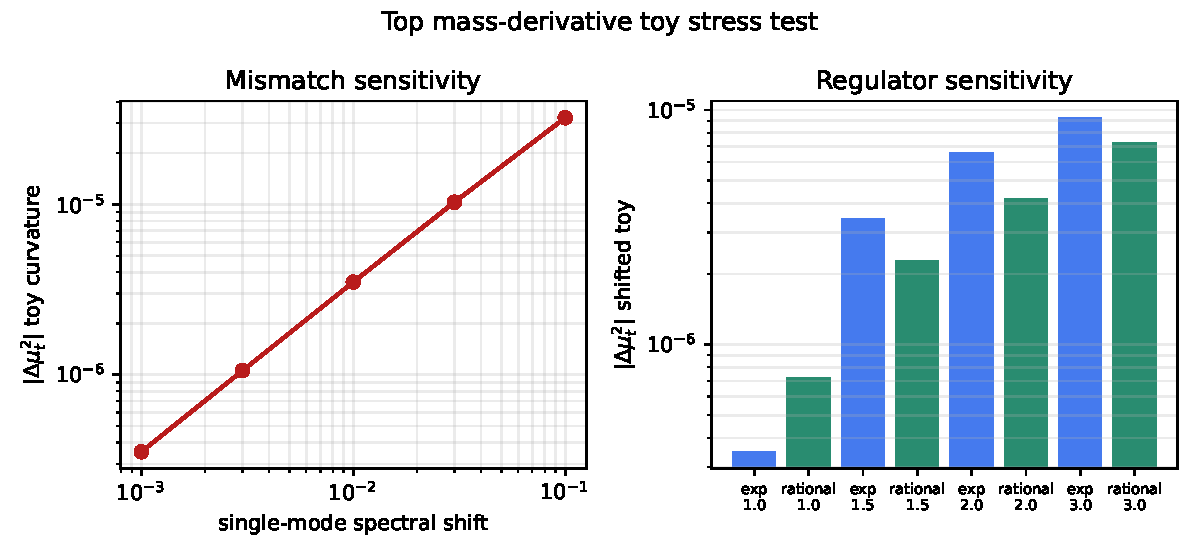
\includegraphics[width=0.92\linewidth]{figures/paper4_top_mass_derivative_toy_stress.pdf}
\caption{Toy top-mass derivative stress test.  Left: a single positive-mode
mismatch induces a growing forbidden curvature.  Right: paired spectra remain
zero under two cutoff families, while shifted spectra leave regulator-dependent
curvature.  This is a diagnostic toy audit, not the physical top determinant,
and is not used as independent evidence for radiative stability.}
\end{figure}

\section{Top Determinant Finite-Residue Extraction Gate}
The previous sections show what must cancel.  The remaining physical question
is narrower: after same-domain positive-mode cancellation, what finite
top-sensitive residue is still admissible?  Define the regulated signed
determinant difference by
\begin{equation}
\Delta\Gamma_t^\Lambda(H)
=
\Gamma_{t,-}^\Lambda(H)-\Gamma_{t,+}^\Lambda(H),
\end{equation}
and subtract the parts already fixed by the paired positive spectrum,
kernel/index sector, anomaly/Ward sector, and boundary sector:
\begin{equation}
R_t^{\rm fin}(H)
=
{\rm FP}_{\Lambda\to\infty}
\left[
\Delta\Gamma_t^\Lambda(H)
-\Delta\Gamma_t^{\rm pos}(H)
-\Delta\Gamma_t^{\rm ind/anom/bdry}(H)
\right].
\end{equation}
Here ${\rm FP}$ denotes the regulator-independent finite part.  The admissible
residue condition is
\begin{equation}
R_t^{\rm fin}
\in
\operatorname{span}\left\lbrace
R_{\rm index},
R_{\rm anomaly},
R_{\rm boundary},
R_{\rm frozen\ matching}
\right\rbrace .
\end{equation}
Any remaining contribution outside this span is not a harmless finite
correction; it is an unaccounted physical term.  In particular, the Higgs-mass
curvature
\begin{equation}
\mu_{t,{\rm fin}}^2
=
\left.
\frac{\partial^2 R_t^{\rm fin}}{\partial H^\dagger\partial H}
\right|_{H=0}
\end{equation}
must vanish, be quotient-null, or be a fixed parent-derived matching residue.
It may not be adjusted after the endpoint is known.  This is the finite-residue
extraction gate: the paper now defines the required computation, but it does
not yet compute the physical $R_t^{\rm fin}$ from a complete parent QFT.

\section{Toy Demonstrator}
The toy demonstrator sets
\begin{equation}
\epsilon_\tau=\mu_\tau({\cal K}_\tau)=N_\tau=C_A=\hat E_{\rm wall}
=\hat M_{\rm stab}=g_{\rm vis}=R_t=1.
\end{equation}
Then
\begin{equation}
m_{\rm toy}=\frac{y_t^{\rm parent}}{\sqrt2}
=0.6799201036561399.
\end{equation}
This is finite and endpoint-free, but it has no GeV interpretation.

\section{Audit Map}
The generated repository checks:
\begin{itemize}
\item the gamma-function quartic overlap and sensitivity scan;
\item Wolfram checks for normalization, hypercharge, line quotient, BRST skeleton, and full-derivation gate-ledger coverage;
\item packet CSV values for $I_4(3/10)$, $0.267097842200176$, $g_t=18/5$, and $y_t^{\rm parent}$;
\item TeX/PDF regeneration and arXiv source package creation;
\item explicit claim-boundary strings in the manuscript.
\end{itemize}

\section{Full Gate Ledger}
\begin{longtable}{p{0.30\linewidth}p{0.58\linewidth}}
\toprule
\textbf{Gate} & \textbf{Current status}\\
\midrule
$3+2$ stabilizer & derived in minimal Branch A carrier\\
$\kappa_\tau^2=3/5$ & canonical hypercharge normalization\\
unoriented line quotient & theorem-candidate with projector audit\\
$\tanh x$ wall & minimal/BPS wall route; parent derivation open\\
$\nu_i=\kappa_\tau^2|Y_i|$ & conditional F1--F8 forcing route\\
quartic overlap & computed: $I_4(3/10)=0.133756368895144$\\
Yukawa overlap & computed: ${\cal I}_{qHu}=0.267097842200176$\\
$g_t$ & bridge-trace candidate $18/5$\\
$y_t^{\rm parent}$ & fixed dimensionless coefficient $0.961552231920634$\\
$v_{\rm eff}$ & stabilizer-gap route, not measured vev derivation\\
$R_t$ & running/matching shape gate\\
$\epsilon_\tau$ & last universal absolute scale blocker\\
wall-cell embedding & same-domain compact-cell requirement\\
top determinant & positive-spectrum cancellation plus finite-residue extraction gate; physical residue not computed\\
BRST/anomaly/regulator & same-domain Ward and trace-cancellation gates formulated; parent complex open\\
Standard Model emergence & roadmap only\\
\bottomrule
\end{longtable}

\section{What Would Count As A Win}
The Higgs route would become much stronger if a single final parent action:
\begin{enumerate}
\item derives the two protected visible modules;
\item derives F1--F8 rather than assuming them;
\item selects ${\cal K}_\tau$ and ${\cal W}_A$ with the required embedding;
\item fixes $\epsilon_\tau$ and $C_A$ without Higgs/top endpoint data;
\item closes the BRST/anomaly/regulator package;
\item computes the physical top finite residue and matching map.
\end{enumerate}

% BEGIN OBSERVER UPDATE 20260914
\section{Observer realization: inherited results and physical boundary}
\label{sec:observer-update-20260914}
The current observer programme distinguishes a conditional mathematical
construction from an occupied physical measuring system. The source order
remains base plus one universal seed, stabilized morphological response,
observer--source restriction, shared descriptor, and resolved terminal
readouts. Neither a detector nor an empirical residual constructs the parent
body backwards. Dynamics below concern downstream subsystems only.

The canonical observer-origin derivation, Sections 22--26, owns the following
results. The existing joint source action fixes static and frequency-dependent
response together. Variation of the BRAC potential couples to the field
square; a linear field coupling is a distinct comparator unless derived by
expansion about an occupied background. Fixed canonical means select a unique
coherent state in a finite positive harmonic packet only if there is no excess
fluctuation energy. This is a free/asymptotic preparation statement, not the
ground state of an interacting detector. For the existing coupled harmonic
pair, the joint ground is pure but either local subsystem is mixed, with its
covariance fixed by the complete joint Hamiltonian.

These are conditional derivations and internal numerical checks. The actual
observer--source context, physical preparation process, kinetic/energy
calibration and stable operational resolution remain unproved. The existing
ORA-T1 selector conditionally chooses stable quantizers when the occupied
context, admissible partition family and positive closure barrier are supplied;
it does not establish those physical premises. A computed ground state is not
a preparation mechanism, and a covariance or optimal abstract measurement is
not an implemented stable quantizer $Q_{OS}$.

\paragraph{Ownership and use.}
The central observer-origin note owns the new contact, state and covariance
derivations; the body-readout technical companion carries the consolidated
mathematics. Foundation Papers IV, V and VI retain physical-selection,
clock-descent and quantum-readout ownership, respectively. This paper imports
only the consequences within its scope. No observational dataset, baseline,
frozen coefficient, score or empirical conclusion is revised by this update.
The reproducibility supplement records the source hashes and the exact
conditional/physical distinction.


\paragraph{Consequence for this paper.}
These results do not select a particle spectrum, coupling constant, Higgs vacuum or gravitational terminal. Common source ancestry remains weaker than physical realization of those sectors.

\subsection{Inherited contact and the occupied-state distinction}
For a positive symmetric three-dimensional quotient $K$, define
$t_K=\operatorname{tr}K$ and $s_K=\operatorname{tr}K^2$. The BRAC shape
invariant and its differential are
\begin{align}
 I_K&=9s_K/t_K^2-3,\\
 dI_K[\delta K]&=\operatorname{tr}
 \left[\left(18K/t_K^2-18s_K\mathbf{1}/t_K^3\right)\delta K\right].
\end{align}
If $K=(LH^{-1}L^*)^{-1}$ on the nonsingular leaf, then
$\delta K=-K\delta(LH^{-1}L^*)K$. Common scaling and orthogonal frame
rotation have zero $dI_K$; the existing spectral-shape control has
$I_K'(0)=-1.06341377025\ldots$. This does not identify its coordinate with
a physical apparatus displacement.

For one real canonically normalized field at fixed coframe and length,
\begin{equation}
 S_K=-\frac12\int \sqrt{-g}\,\frac{I_K}{\ell_H^2}\phi^2\,d^4x,
 \qquad b_j=\ell_H^{-2}dI_K[\partial_{a_j}K].
\end{equation}
The corresponding potential interaction is
$H_{\rm int}=\sum_j a_j B_j$ with
$B_j=\frac12\int b_j\phi^2\,d^3x$. The actual subsystem pullback,
kinetic terms and calibration remain required. For a free real scalar in
a stationary inertial vacuum the Wick-square correlation is $2W^2$,
so this contact has a two-quantum threshold $2\nu_B$, not the linear
comparator's $\nu_B$. With $c=\hbar=\ell_H=1$, $m_0=0$ and the
source CHDF value $I_K=0.0610078751932586$, the thresholds are
$0.24699772305278$ and $0.49399544610556$. The previous comparison gaps
$0.35$ and $0.15$ therefore have different support in the two contact models.
Neither threshold is asserted for arbitrary trajectories or occupied states.

For a supplied coherent background, mean force and connected covariance
follow from the same contact:
\begin{align}
 \langle B_i\rangle&=\frac12\int b_i\phi_{\rm cl}^2\,d^3x,\\
 C_{ij}(t,t')&=\int d^3x\,d^3y\,b_i(x)b_j(y)
 \left[\phi_{\rm cl}(t,x)\phi_{\rm cl}(t',y)W(t,x;t',y)
 +\frac12 W(t,x;t',y)^2\right].
\end{align}
Vacuum Wick ordering here is a comparison prescription, not a derivation
of the physical stress renormalization. A nonzero classical mean does not
by itself select this quantum state. The kernel is a free interaction-picture
input, generally nonstationary, not an all-orders interacting bath law.

\subsection{Conditional state selection and its resource requirement}
For a supplied finite positive oscillator packet, fixed means
$\operatorname{Tr}(\rho c_r)=\alpha_r$ imply
\begin{equation}
 \langle H_{\rm exc}\rangle=
 \sum_r\hbar\omega_r|\alpha_r|^2+
 \sum_r\hbar\omega_r
 \langle(c_r-\alpha_r)^\dagger(c_r-\alpha_r)\rangle.
\end{equation}
The second sum is nonnegative. Equality with the classical mean energy
forces the state into the common kernel of all $c_r-\alpha_r$, hence the
unique coherent state. With excess energy $\Delta E$,
\begin{equation}
 1-\langle\alpha|\rho|\alpha\rangle
 \leq \frac{\Delta E}{\hbar\omega_{\min}}.
\end{equation}
Displaced number states have the same means and higher energy, providing
an explicit counterexample when the zero-excess condition is omitted.
Ground-state minimization does not provide autonomous preparation.
For energy-calibrated amplitude $\psi_E$, the source-preserving displacement
is $\alpha=(2\hbar\Omega)^{-1/2}\psi_E$. If the input is action-normalized,
the energy/clock conversion remains necessary; it cannot be replaced by
setting every mode frequency to one.

For a declared common-frame tetrahedral coherent code, equal priors and
$\alpha_i=\sqrt{N}n_i$, $n_i\cdot n_j=-1/3$, the off-diagonal overlap is
$s=\exp(-4N/3)$. The exact optimal single-shot discrimination probability is
\begin{equation}
 P_{\rm opt}=\frac{[\sqrt{1+3s}+3\sqrt{1-s}]^2}{16}.
\end{equation}
The square-root measurement attains this value. With $S=\sqrt{G}$ and
$d=S_{ii}$, the dual operator $Y=dS/4$ has matching trace and
$Y-v_iv_i^*/4\succeq0$ for columns $v_i$ of $S$, proving optimality.
Uniform pure loss replaces $N$ by $\eta N$ only in that declared channel
model. This coherent code is not the earlier one-particle leaf encoding;
the bound does not construct a physical receiver or stable $Q_{OS}$.

\subsection{Joint coupling fixes local uncertainty}
The existing two-copy action, expanded at an already aligned local well,
has $H=\left(\begin{smallmatrix}D&-C\\-C^T&D\end{smallmatrix}\right)$,
$D=e_*(S_i+16\mathbf1)$, $C=16e_*\mathbf1$ and
$S_i=3P_i+4(\mathbf1-P_i)$. Given a positive kinetic matrix $G$,
canonical quantization and joint harmonic ground preparation, put
$W=(G^{-1/2}HG^{-1/2})^{1/2}$. Normal-mode diagonalization gives
\begin{equation}
 V_z=\frac\hbar2G^{-1/2}W^{-1}G^{-1/2},\qquad
 V_p=\frac\hbar2G^{1/2}WG^{1/2}.
\end{equation}
For equal inertia $I_0$, a ray of curvature $s_0=3,4$ has frequencies
$\omega_c^2=e_*s_0/I_0$ and $\omega_r^2=e_*(s_0+32)/I_0$. Its local
symplectic eigenvalue is
\begin{equation}
 \nu_{s_0}=\frac14\sqrt{2+\omega_r/\omega_c+\omega_c/\omega_r}>\frac12.
\end{equation}
The joint state is pure but the equal-inertia three-mode local purity is
$0.627817314635553$. The local position covariance also equals
\begin{equation}
 V_x=\frac\hbar\pi\int_0^\infty
 \left[D+I_0\xi^2\mathbf1-C(D+I_0\xi^2\mathbf1)^{-1}C^T\right]^{-1}d\xi.
\end{equation}
Thus the full frequency-dependent Schur kernel, not its static value followed
by a local vacuum assignment, determines the fluctuations. For dimensionless
coordinates, $H$ has energy units, $G$ energy-times-time-squared units, and
$\hbar/\sqrt{I_0e_*}$ controls fluctuation size.

The unit-scale Gaussian has only $0.18974552836899916$ probability inside
the previously declared radius $\sqrt{8/3}/4$ about the chosen vertex.
That control does not certify localized records. The state is a local
quadratic-well ground, not the full nonlinear multiwell ground or the
outcome of a preparation process. Its copies have not been physically
identified with the BRAC observer. An adopted acceptance ball is not a
source-selected stable quantizer or a measured efficiency.

\paragraph{Scientific status.}
The canonical calculations supply exact conditional identities and finite
numerical controls, not Nature occupation. Physical observer identification,
preparation, nonlinear record stability and calibrated operational resolution
remain open. Standard quadratic-detector, coherent-state and coupled-Gaussian
physics supply comparison methods, not evidence of a Tau-specific effect.
% END OBSERVER UPDATE 20260914

\section{Conclusion}
The full derivation ledger shows that the Higgs branch has moved from a single
quartic coincidence to a structured single-package proof program.  The sharp
fixed chain is
\begin{equation}
3+2
\rightarrow
\kappa_\tau^2=\frac35
\rightarrow
\nu_H=\frac3{10}
\rightarrow
I_4(3/10)
\rightarrow
{\cal I}_{qHu}
\rightarrow
 y_t^{\rm parent}=0.9615522319206335.
\end{equation}
The remaining blockers are now also sharp: $\epsilon_\tau$, $C_A$, compact cell,
wall embedding, continuum regulator, top determinant, and matching.  Until
those are derived, this is a disciplined candidate derivation program, not a
completed Higgs-sector proof.

Negative status at closure: conditional compact spectral theorem and
parent-domain selection functional formulated within stated operator-domain
assumptions, but exhaustive domain classification is not closed; conditional
positive-spectrum determinant cancellation follows within the same-domain
setup and finite-residue extraction gate is formulated, but no computed
physical top finite residue;
conditional anomaly/Ward and representation trace-cancellation gates
formulated, but no computed parent-derived representation complex;
UV/continuum admissibility criterion and microscopic completion target
formulated, but no convergent parent action family; physical matching map and
endpoint protocol formulated, but no numerical endpoint matching yet.

\end{document}
